%%%%%%%%%%%%%%%%%%%%%%%% Title Page %%%%%%%%%%%%%%%%%%%%%%%%
\documentclass[12pt, a4paper, titlepage]{article}
\usepackage[a4paper,left=2.5cm,right=2.5cm,top=2.54cm,bottom=2.54cm]{geometry}
\usepackage{float}
\usepackage{lipsum}
\usepackage{placeins}
\usepackage[bottom]{footmisc}
\usepackage{float}
\usepackage[hidelinks]{hyperref}
\usepackage{graphicx}
\usepackage{appendix}
\usepackage{setspace}
\usepackage{dcolumn}
\usepackage[printonlyused, withpage]{acronym}
\usepackage{amsmath}
\usepackage{xcolor}
\DeclareMathOperator*{\argmax}{arg\,max} 
\usepackage{natbib}
\makeatletter
\newcommand{\MSonehalfspacing}{%
  \setstretch{1.44}%  default
  \ifcase \@ptsize \relax % 10pt
    \setstretch {1.448}%
  \or % 11pt
    \setstretch {1.399}%
  \or % 12pt
    \setstretch {1.433}%
  \fi
}
\newcommand{\MSdoublespacing}{%
  \setstretch {1.92}%  default
  \ifcase \@ptsize \relax % 10pt
    \setstretch {1.936}%
  \or % 11pt
    \setstretch {1.866}%
  \or % 12pt
    \setstretch {1.902}%
  \fi
}
\makeatother
\MSonehalfspacing

\usepackage{listings}
\usepackage{xcolor}

\newenvironment{acknowledgments}{%
  \renewcommand*{\abstractname}{Acknowledgments} \abstract}{%
  \endabstract
}

\newenvironment{ConflictofInterest}{%
  \renewcommand*{\abstractname}{Conflict of Interest Statement} \abstract}{%
  \endabstract
}


\colorlet{punct}{red!60!black}
\definecolor{background}{HTML}{EEEEEE}
\definecolor{delim}{RGB}{20,105,176}
\colorlet{numb}{magenta!60!black}

\lstdefinelanguage{json}{
    basicstyle=\normalfont\ttfamily,
    numbers=left,
    numberstyle=\scriptsize,
    stepnumber=1,
    numbersep=8pt,
    showstringspaces=false,
    breaklines=true,
    frame=lines,
    backgroundcolor=\color{background},
    literate=
     *{0}{{{\color{numb}0}}}{1}
      {1}{{{\color{numb}1}}}{1}
      {2}{{{\color{numb}2}}}{1}
      {3}{{{\color{numb}3}}}{1}
      {4}{{{\color{numb}4}}}{1}
      {5}{{{\color{numb}5}}}{1}
      {6}{{{\color{numb}6}}}{1}
      {7}{{{\color{numb}7}}}{1}
      {8}{{{\color{numb}8}}}{1}
      {9}{{{\color{numb}9}}}{1}
      {:}{{{\color{punct}{:}}}}{1}
      {,}{{{\color{punct}{,}}}}{1}
      {\{}{{{\color{delim}{\{}}}}{1}
      {\}}{{{\color{delim}{\}}}}}{1}
      {[}{{{\color{delim}{[}}}}{1}
      {]}{{{\color{delim}{]}}}}{1},
}

\usepackage{caption}
\usepackage{subcaption}

%%%%%%%%%%%%%%DOCUMENT%%%%%%%%%%%%%%
\begin{document}
%%%%%%%%%%%%%%TITLEPAGE%%%%%%%%%%%%%%
\begin{titlepage}
    \begin{center}
    {\LARGE \textbf{Job Title Classification}}
    \noindent\rule[0.5ex]{\linewidth}{1pt}
    {\Large \textbf{A Comparision of Vectorization and Classification Techniques for German Job Postings}}
    \\[1cm]
    {\Large \textbf{Masterthesis}}
    \\[1cm]
    {\normalsize A thesis submitted in partial fulfilment of the requirments for the degree of the Master of Social and Economic Data Science at the University of Konstanz}
    \\[1cm]
    {\Large submitted by}
    \\[0.5cm]
    \renewcommand*{\thefootnote}{\fnsymbol{footnote}}
    {\Large \textbf{Rahkakavee Baskaran}\footnote{Contact details: Howiesenstraße 5, 70839 Gerlingen, rahkakavee.baskaran@uni-konstanz.de}}
    \\[0.5cm]
    {\Large 01/950253}
    \\[0.5cm]
    {\Large at}
    \\[1cm]
    
\includegraphics[width=0.6\textwidth]{logo.jpg}
    \\[1cm]
    {\normalsize \textbf{Period of completion: October, 8, 2021 - Februrary, 15, 2022}} 
    \\[0.2cm]
  {\normalsize \textbf{1\textsuperscript{st} supervisor:} Professor Doctor Susumu Shikano}
  \\[0.1cm]
  {\normalsize \textbf{2\textsuperscript{nd} supervisor:} Junior Professor Juhi Kulshresthra}
  \\[1cm]
    {\Large \textbf{Konstanz, \today}}
  \end{center}
    \end{titlepage}

%%%%%%%%%%%%%%TableOfContents%%%%%%%%%%%%%%
\tableofcontents
\newpage
\listoffigures
\newpage
\listoftables
\newpage
%%%%%%%%%%%%%%Abbreviations%%%%%%%%%%%%%%
\section*{Abbreviations}
\begin{acronym}
  \acro{BERT}[BERT]{Bidirectional Encoder Representations from Transformers}
  \acro{BOW}[BOW]{Bag of Words}
  \acro{CBOW}[CBOW]{Continous Bag of Words}
  \acro{CNN}[CNN]{Convolutional Neural Network}
  \acro{CART}[CART]{Classification and Regression Trees}
  \acro{DF}[DF]{Document Frequency}
  \acro{FN}[FN]{False Negatives}
  \acro{FP}[FP]{False Positives}
  \acro{IDF}[IDF]{Inverse Document Frequency}
  \acro{ISCO}[ISCO]{International Standard Clasification of Occupations}
  \acro{KldB}[KldB]{Klassifikation der Berufe 2010}
  \acro{KNN}[KNN]{K-Nearest-Neighbor}
  \acro{LR}[LR]{Logistic Regression}
  \acro{MAP}[MAP]{Maximum a Posteriori}
  \acro{NLP}[NLP]{Nature Language Processing}
  \acro{NB}[NB]{Naive Bayes}
  \acro{OA}[OA]{Overall Accuracy}
  \acro{PCA}[PCA]{Principal Component Analysis}
  \acro{RF}[RF]{Random Forest}
  \acro{RNN}[RNN]{Recurrent Neural Networks}
  \acro{SVM}[SVM]{Support Vector Machine}
  \acro{TF}[TF]{Term Frequency}
  \acro{TF-IDF}[TF-IDF]{Term Frequency-Inverse Document Frequency}
  \acro{TP}[TP]{True Positives}
  \acro{TN}[TN]{True Negatives}
\end{acronym}
\newpage

\begin{acknowledgments}
I would like to express my sincere gratitude to my supervisors Professor. Dr. Susumu Shikano and Junior Professor Juhi Kulshresthra, who guided me throughout this project.

\bigskip

\noindent My special thanks go to Johannes Müller and his team at cause\&effect DFSG UG for their guidance during the thesis, as well as for providing the data.

\bigskip

\noindent Lastly, I would also like to thank my family and friends for their encouragement and support throughout my thesis. 
\end{acknowledgments}

\begin{abstract}
  Job titles are key information within the area of labor market. As a valuable resource for labor market analysis and an essential component of job search engines and job recommendation systems, it is necessary to develop classification systems for job titles based on taxonomies that reflect current market trends. So far, the literature has focused on the English-speaking job market, while there are no classification attempts for the German market. Therefore, this work aims to compare different vectorization and classification methods for the classification of German job titles, taking into account one of the challenges of this task, namely the classification of short texts. The comparison is made using the five vectorization techniques count vectorizer, TF-IDF, word2vec, doc2vec, and BERT. The data is trained using LR, SVM, and RF. In addition, a BERT deep learning model is applied. Word2vec and doc2vec are additionally tested with additional knowledge to account for short text classification issues. The results show that BERT as a vectorization technique is a promising method for classifying German occupational titles. It is stable and offers excellent performance in classifiying imbalanced data and compared to other methods. The inclusion of additional knowledge into the classification of short job titles, however, yields inconclusive results.
\end{abstract}


%%%%%%%%%%%%%%SECTIONS%%%%%%%%%%%%%%
\section{Introduction}
Job titles are key information within the area of labor market. They are helpful for job seekers to find jobs \citep{marinescu2020}; they are an essential component of job search engines \citep{slamet2018, javed2015, javed2016} and job recommendation systems \citep{malherbe2014}; and lastly, they serve as a valuable data source for various analyses, such as job market trends \citep{martin2021, li2021}, job perception \citep{smith1989, boydston2020} or social science analyses \citep{martin2021}. However, since job titles are not normalized, it is challenging to structure them appropriately for downstream tasks. Various institutions developed job taxonomies to structure and generalize job titles. Established taxonomies are, for example, the \ac{ISCO} for the European job market or the \ac{KldB} for the German job market \citep{uter2020}. Classifying job titles from job postings into classes based on these taxonomies is indispensable to improve job search engines or recommendation systems or to enable comprehensive analysis of the labor market. 

In the literature, there exist some works on the classification of job titles \citep{zhu2016, javed2015, decorte2021, wang2019,neculoiu2016}. While job title classification systems like ``Carotene" \citep{javed2015} have been developed for English job titles, to the best of my knowledge, there have not been any classification attempts for German titles yet. However, accurate classification of job titles with the \ac{KldB} taxonomy would facilitate several downstream tasks for the German job market. With the \ac{KldB} 2010, a taxonomy was created that reflects the current trends in the labor market based on empirical and theoretical foundations, which gives an excellent basis for the normalization. In addition, most previous work does not have a solid database due to the lack of labeled data. This often leads researcher to resort to unsupervised methods \citep{decorte2021, javed2015}. For the German job market, the Federal Employment Agency provides job postings with labeled titles on their job board, creating large labeled data for text classification. 

Over time, the literature on \ac{NLP} has been virtually flooded with algorithms for text classification. Starting with traditional techniques followed by ensemble techniques, nowadays, deep learning methods dominate the research. Choosing a classification algorithm is far from trivial: no algorithm works equally well for every task. This makes exploration and comparison of different algorithms necessary. However, not only the choice of the classifier itself is challenging, but also the input for the algorithms plays a significant role. Methods have been developed that take into account various properties, such as the context of the text or the consideration of word order. This results in vectors with different densities and dimensions. In order to develop a powerful algorithm, various techniques have to be explored and compared.

Task-specific requirements necessitate further adjustments in the training process. The focus of this paper is on the challenge of job titles being concise. Short texts suffer from sparseness, few word co-occurrences,  missing shared context, noisiness, and ambiguity. The literature offers several approaches. Enriching features with additional knowledge has proven to be a promising method \citep{WangF2014, wang2017J}.

Given the lack of a classification system for German job titles and the challenges this task entails, I define the following research goal: A comparison of different vectorization and classification methods for classifying German job titles under consideration of short text classification. The comparison should help to develop a German job title classification system based on the \ac{KldB} taxonomy to facilitate downstream tasks for the German labor market. Based on the state of the literature, the comparison is carried out under three aspects: First, different feature extraction techniques are implemented and compared. The comparison includes the sparse vectors count vectorizer and \ac{TF-IDF} and the dense techniques word2vec, doc2vec, and \ac{BERT}. Second, different classifiers from different research directions are considered. The traditional methods \ac{SVM} and \ac{LR}, the ensemble technique \ac{RF}, and \ac{BERT} as a deep learning method are applied and compared. Finally, the task-specific challenge of short texts is considered by enriching word2vec and doc2vec, each with a second model with additional knowledge from the taxonomy. 

Some interesting trends emerge from the training. \ac{BERT} as a vectorization technique is the clear winner. The sparse vectors perform better than word2vec and doc2vec, except for \ac{RF} where word2vec has similar performance to the sparse vectors. Except for \ac{BERT}, the other classifiers developed label bias in different settings, which explains most of the performance scores. The additional knowledge may have positively affected the word2vec embedding technique, while it may have been detrimental to doc2vec. 

This paper is structured as follows: The first section gives an overview of the related work to derive the research gap and the framework for the task. The following section presents the datasets and elaborates on the taxonomy. This is followed by the third chapter, with a detailed explanation of the pipeline and the associated methods. In a next step the results are presented. Finally a conclusion is drawn at the end of the paper and limitations are pointed out. 

\section{Related Work}
\paragraph{Job Title Classification}
For the English job market, there are already some studies dealing with job title classification. In terms of classifiers, the corresponding work can be categorized into traditional classifiers or deep learning methods. \cite{zhu2017} for example, use a \ac{KNN} classifier in combination with document embedding as a feature selection strategy. \cite{javed2015} rely on traditional methods as well, by combining a \ac{SVM} classifier and a \ac{KNN} classifier for their job recommendation system. In contrast, the approaches of \cite{decorte2021}, \cite{wang2019} and \cite{neculoiu2016} are based on deep learning methods. From a differentiated framework perspective, there is another dividing line between the approaches. As mentioned earlier, job title normalization can be considered a typical text classification task \citep{wang2019, javed2015, zhu2017}. \cite{decorte2021} and \cite{neculoiu2016}, however, formulate the task as a string representation approach of similar job titles. 

While there is some work on job title classification for the English speaking job market, to the best of my knowledge, there have not been any classification attempts for the German job market. However, an accurate classification of job titles with the German \ac{KldB} taxonomy would facilitate several downstream tasks for the German job market. Besides the lack of a classification system, most of the work on job title classification suffers from the lack of solid databases. Therefore, \cite{decorte2021}, for example, use skills mentioned in job advertisements to understand the meaning of job titles and to avoid manually labelling them. \cite{javed2015} rely on a weakly supervised approach to get enough labelled data. The advantage of classifying for the German job market is that the Federal Employment Agency of Germany provides a dataset with job titles and the possibility of linking them with die \ac{KldB} classes, which offers a huge and powerful training dataset which in turn allows for more flexibility in which algorithms are applicable. Following \citet{wang2019, javed2015, zhu2017} the task will be framed as a text classification task. 

\paragraph{Text Classification Algorithms}
During the last decades, researchers developed a various number of classifiers. In their survey of classifiers, \cite{kowsari2019text} differentiate between three groups of approaches. The first group contains traditional methods like \ac{NB}, \ac{SVM}, \ac{KNN}, \ac{LR} or Decision Trees \citep{Vijayan2017, Colas2006, kowsari2019text, Sebastiani2001}. Deep learning methods like \ac{CNN} or \ac{RNN}, which are currently the most advanced algorithms for \ac{NLP}, form the second group. The last group consists of ensemble learning techniques like Boosting and Bagging. Each group can be further split mainly into supervised and unsupervised learning techniques. Since labeled data is available for the classification task in this study, the focus will be on supervised learning techniques. 

Classification algorithms can be selected on different criteria. Certainly, one of the most important criteria is performance. Currently, deep learning methods often outperform traditional methods and ensemble techniques. Deep Learning methods are advanced methods of traditional machine learning algorithms. In contrast to traditional methods, they do not require a substantive understanding of feature extraction since they automatically extract important features. Many comparative studies on traditional and embedding techniques vs.\ deep learning text classification tasks show the strength of deep learning. \citet{wang2017} compared \ac{SVM} and \ac{KNN} for web text classification against \ac{CNN}. Their results reveal a better performance of \ac{CNN} over the traditional methods. \citet{hassan2017} likewise show that \ac{CNN}, but also \ac{RNN} outperform traditional methods with \ac{BOW} feature extraction. These results are corroborated by \citet{kamath2018}. Furthermore, \citet{gonzalez2020} compared the current state-of-the-art deep learning model \ac{BERT} with traditional methods using the \ac{TF-IDF} feature selection method and show clear outperformance by \ac{BERT}. 

Although deep learning models often outperform traditional methods in these comparative studies, not all classifiers achieve good results over all applications. In contrast to traditional methods, deep learning models also usually require millions of data to train an effective model \citep{chauhan2018}. Thus, deep learning methods are not necessarily always the right choice. For example, \citet{zhang2015}, conducted experiments on character-level \ac{CNN} and compared them to different traditional models, like \ac{BOW} or Bag of Ngrams with \ac{TF-IDF} and \ac{LR}. For smaller and moderate size news datasets, the traditional methods, except for Bag of Means, performed well, and some of them outperformed \ac{CNN}. For bigger datasets, \ac{CNN} worked better. Another study from \citet{yan2018} relies on a siamese \ac{CNN} deep learning approach with few-shot learning for short text classification using different Twitter benchmark data. They compared their results to some baseline deep learning methods and traditional methods, including \ac{SVM}, ensemble techniques, and \ac{LR}. Although the siamese \ac{CNN} outperformed all the other methods clearly, some traditional methods outperformed the baseline deep learning methods for specific datasets.  

Comparisons of ensemble techniques, traditional methods, and methods within the traditional methods indicate that not all classifications perform equally good or poor for all tasks. A comparative analysis with \ac{LR}, \ac{RF} and k-nearest neighbor, using \ac{TF-IDF}, for news text classification indicates a good performance of \ac{LR} and \ac{RF} compared to \ac{KNN}, wherby \ac{LR} performed better then \ac{RF} \citep{shah2020}. A study from biomedical classification shows that among \ac{RF}, \ac{NB} with \ac{TF-IDF} and \ac{SVM} the best performance was achieved by \ac{SVM} \citep{danso2014}. 

Although performance is essential, other criteria like the transparency of the algorithm, the interpretability, and efficiency in terms of the runtime are not irrelevant. Methods like \ac{NB} or \ac{LR} are much faster than neural networks or \ac{SVM}s. In terms of transparency and interpretability, algorithms like Decision Tree or \ac{LR} are more intuitive and easier to understand and interpret. In contrast, deep learning models and \ac{SVM} rely on more complex computations. Especially deep learning lacks transparency \citep{maglogiannis2007}. As for \ac{BERT}, although it usually outperforms other machine learning algorithms for text classification, in general ``there are more questions than answers about how \ac{BERT} works" \citep[853]{rogers2020}. It is, for example, not well-understood so far what exactly happens during the fine-tuning process of \ac{BERT} \citep{merchant2020}. In spite of the other qualification criteria, the main focus of this analysis is on performance. 

\paragraph{Vectorization Methods}
Besides the classifier, it is also important for the performance with which inputs the classifiers are fed. Texts must be converted into a numerical representation to make them machine-readable \citep{singh2019}. The numerical vector representations of a text or document can be divided into sparse and dense vectors, also called word embeddings. Sparse vectors, relying on the \ac{BOW} model, are high-dimensional vectors with many zeros, while word embedding techniques have a fixed-length representation \citep{almeida2019}. Sparse vectors are for example \ac{TF-IDF} or count vectorizer. Examples for word embedding techniques are word2vec, doc2vec, and \ac{BERT}. 

Unsuitable features considerably affect the performance of the classification algorithms \citep{cahyani2021}. The correct selection of a feature extraction technique depends on many factors, like the length of the dataset or the specific domain \citep{arora2021}. Empirically, this is reflected in the diverse and conflicting studies in the literature. Considering the sparse vectors, \citet{wendland2021} compared for fake news data \ac{TF-IDF} and count vectorization. While they found slightly better results with \ac{TF-IDF}, the results of \citet{WangY2017} show no difference between them. Some studies from different domains demonstrate the strength of word2vec compared to \ac{TF-IDF} \citep{arora2021, rahmawati2016}, while others show opposite results \citep{zhu2016,cahyani2021}. \citet{shao2018} conclude that they find no clear picture between \ac{BOW} models and word2vec. Comparing doc2vec and word2vec, \citet{lau2016} found in general good performance of doc2vec. However, the authors admit that the qualitative differences between both techniques are not clear. Both \citet{shao2018} and \citet{WangY2017} obtain the worst results for doc2vec compared to word2vec and \ac{BOW} vectorization techniques. \ac{BERT} shows overall a good performance \citep{gonzalez2020}. Nevertheless, \citet{miaschi2020} conclude from their research finding that word2vec and \ac{BERT} code similarly for sentence-related linguistic features.  

\paragraph{Challenges of Job Title Classification}
Each text classification task has different challenges. One challenge of the presented task is the number of classes. As \cite{li2004} show in their classification of tissue, multi-class classification is more complex than binary classification problems. Partly because most classification algorithms were designed for binary problems \citep{aly2005}. Approaches for multi-class classification can be grouped into two types. Either binary algorithms can handle multi-class classification naturally, or the problem is decomposed into binary classification tasks \footnote{for the different subtypes, see \cite{aly2005}}. The literature so far does not have a clear answer to solve multi-class classification problems. Different approaches, like boosting \citep{schapire2000} or \ac{CNN} \citep{farooq2017} are applied. It is apparent, however, that many works use variations of \ac{SVM} \citep{guo2015, tomar2015comparison, Tang2019}.  

Another important issue for text classification is the length of input documents. Job titles are short texts with often not more than 50 characters. Short texts suffer from sparseness, few word co-occurrences, missing shared context, noisiness, and ambiguity. These attributes make it challenging to construct features that capture the meaning of the text. Furthermore, traditional methods are based on word frequency, high word co-occurrence, and context, which is why they often fail to achieve high accuracy for short texts \citep{Song2014, WangY2017, WangF2014,  alsmadi2019}. Besides this, short texts are also often characterized as having a lot of misspelling and informal writing. The last two attributes of short texts are indeed a problem, e.g., for Twitter data, which is a popular topic for short text data \citep{karimi2013, sriram2010, yan2018}. However, these attributes play little or no role in the job title classification, especially compared to the other stated issues, since job postings are usually reviewed and controlled thoroughly before release. Due to this, only research concerning the first mentioned attributes is considered in the following. 

A popular approach proposed by many researchers for improving short text classification is to add additional knowledge to the features. Many studies of Twitter short texts demonstrate the power of this approach. \citet{karimi2013}, for example, use a \ac{BOW} approach for disaster classification of Twitter posts. They experiment with different features enriched by additional information. While, for example, generic features like the number of hashtags improved classification, other information like incident-specific features only helped in specific settings. All in all, the use of \ac{BOW} with specific features delivers quite good performance. Similarly, \citet{sriram2010} achieved a good performance for Twitter short text messages, using features extracted manually from the short text itself.

Criticism of the \ac{BOW} approach for short text classification is raised by \citet{WangF2014} since \ac{BOW} results usually in high dimensional data. They state that this is much more harmful to short texts because they are short and sparse. They propose a ``bag of concept" approach using a knowledge base. The knowledge base is used to learn concepts for each category and find a set of relevant concepts for each short text. Following this, \citet{wang2017J} use an enriching concept for short text classification. They use a concept vector combined with a taxonomy knowledgebase which indicates how much a text is related to the concept. Those are merged with the word embeddings. In addition, they add character-level features. 

In general, in short text classification, the question arises whether to represent the features as dense or sparse vectors. Based on their comparison of \ac{TF-IDF} and the count vectorizer against the dense vectorizer word2vec and doc2vec, \cite{WangY2017} conclude that among the classifiers \ac{NB}, \ac{LR} and \ac{SVM}, the sparse vectorizers achieve the highest accuracy. \cite{Chen2019}, conversely, see limitations in sparse representation as it cannot capture the context information. In their work, they integrate sparse and dense representation into a deep neural network with knowledge-powered attention, which outperforms state-of-art deep learning methods, like \ac{CNN}, for Chinese short texts. 

In contrast to the above mentioned approaches, \citet{sun2012} pursues a completely different strategy. Instead of enriching the features, he focused them on specific keywords. In order to select the essential keywords, he used \ac{TF-IDF} approaches, some with a clarity function for each word. Using \ac{LR} he accomplished persuasive results for his classification.

Instead of feature enrichment according to \citet{Song2014}, some researchers also apply feature dimensionality reduction and extraction of semantic relationship techniques using, for example, Latent Dirichlet approaches.

Concerning the classifiers, there is no consensus approach for short text classification. For traditional approaches, the results of \cite{WangY2017} indicate that \ac{LR} and \ac{SVM} perform best, while \cite{Khamar2013} displays that \ac{KNN} has the best achieved accuracy. \citet{Song2014} propose to use ensemble techniques. In combination with enriched features \citet{Bouaziz2014}, for example, achieve better results as for \ac{LR} with ensemble techniques. Similar to job title-specific work, more recent work prefers deep learning methods, mostly \ac{CNN} \citep{Chen2019}. 

\paragraph{Implications of State of Research}
There are three consequences emerging from the above-discussed literature. Firstly, appropriate feature selection or vectorization plays a decisive role in the performance. For that reason, I implement several feature extraction techniques covering sparse and dense vectors. For sparse vectors, I transform the data with count vectorizer and \ac{TF-IDF} vectorizer. Word2vec, doc2vec, and \ac{BERT} embedding built the group of dense vectorization techniques. The discussion of the different techniques will be the first pillar of the comparison. 

Secondly, relying on one classification does not seem to be a reasonable option. Instead, experimenting and exploring different traditional, deep learning, and ensemble classifiers allows for identifying the best classifier based on the task and the data \citep{maglogiannis2007}. Therefore, I use four classifiying techniques. Two of them are traditional methods. The literature shows that \ac{SVM} and \ac{LR} are well compatible with other techniques, which is why I choose both of them. I also include \ac{RF} as an ensemble technique. As the last method, I implement a \ac{BERT} deep learning model since it is the state-of-art method for text classification. The evaluation of different classifications builds the second pillar of the comparison. 

Thirdly, from the two challenges presented, the focus of this paper is on the classification of short texts. The literature on short text classification reveals two issues. First, there are different results on whether sparse or dense techniques are better suited. Testing different sparse and dense vectorization techniques allows adressing this issue. Second, most of the solutions include additional knowledge. Therefore, I introduce a second model for each word2vec and doc2vec with additional knowledge from the taxonomy. The model comparison between these models forms the last pillar of the comparison. 


\begin{table}[]
  \resizebox{\textwidth}{!}{%
  \begin{tabular}{cl}
  \hline
  \multicolumn{1}{l}{\textbf{IDs KldB 2010}} & \textbf{Berufsbereich (Level 1)}                                           \\ \hline
  1                                          & Land-, Forst- und Tierwirtschaft und Gartenbau                             \\
  2                                          & Rohstoffgewinnung, Produktion und Fertigung                                \\
  3                                          & Bau, Architektur, Vermessung und Gebäudetechnik                            \\
  4                                          & Naturwissenschaft, Geografie und Informatik                                \\
  5                                          & Verkehr, Logistik, Schutz und Sicherhe                                     \\
  6                                          & Kaufmännische Dienstleistungen, Warenhandel, Vertrieb, Hotel und Tourismus \\
  7                                          & Unternehmensorganisation, Buchhaltung, Recht und Verwaltung                \\
  8                                          & Gesundheit, Soziales, Lehre und Erziehung                                  \\
  9 & Sprach-, Literatur-, Geistes-, Gesellschafts- und Wirtschaftswissenschaften, Medien, Kunst, Kultur und Gestaltung \\
  0                                          & Militär                                                                    \\ \hline
  \end{tabular}%
  }
  \caption[Overview of Classes Level 1 - Berufsbereiche]{\label{tab: T3} Overview of Classes Level 1 - Berufsbereiche (adapted from \citep[9]{Bundesagentur2011a} and \citep[1]{Bundesagentur2011b})}
  \end{table}


\section{Job Title Data and Taxonomy}
\setcounter{footnote}{0}
The training data consists of two datasets.\footnote{Both datasets are provided by cause\&effect DFSG UG for this study. They are not publicly available in this format.} The classes are extracted from the first dataset, referred to below as the \ac{KldB} dataset. The \ac{KldB} dataset contains all information of the \ac{KldB} taxonomy. The second dataset, called the job title dataset, contains the necessary data from the job titles. In the first part of this chapter, a brief explanation about the taxonomy structure and both datasets is given. The second part consists of a descriptive analysis of the class distribution of the data. 

\subsection{KldB 2010}
The \ac{KldB} dataset is structured hierarchically with five levels, with each level containing a different number of classes. The classifiers are trained for level 1 and level 3. In the following, these classes are also referred to as \textit{kldb}. On level 1, each class has an id of length 1 with a number from 0 to 9. Table \ref{tab: T3} shows the ten classes of level 1 with their class names. On level 2, each of the ten classes is divided into one or more subclasses having a class id of length 2, with the first digit indicating the class of level 1 and the second digit the class of level 2. An overview of all five levels with an example of classes is given in table \ref{tab: T2}. This procedure ultimately leads to class ids of length five on level 5. An occupation can be classified on every level in the taxonomy. Considering the classes of the example in table \ref{tab: T2}, the job title ``java developer" could be classified on level 5 to the class 43412. From this id, it is also derivable that the job title belongs, for example, on level 3 to the class ``Sofwareentwicklung" \citep{Bundesagentur2011a, Bundesagentur2011b, Paulus2013}.

  \begin{table}[]
    \center
    \resizebox{\textwidth}{!}{
    \begin{tabular}{lccl}
    \hline
    \textbf{Name}      & \textbf{Level} & \textbf{Number of Classes} & \textbf{Example}                               \\ \hline
    Berufsbereiche     & 1              & 10                         & 4: Naturwissenschaft, Geografie und Informatik \\
    Berufshauptgruppen & 2 & 37   & 43: Informatik-, Informations- und Kommunikationstechnologieberufe            \\
    Berufsgruppen      & 3              & 144                        & 434: Sofwareentwicklung                        \\
    Berufsuntergruppen & 4              & 700                        & 4341: Berufe in der Sofwareentwicklung         \\
    Berufsgattungen    & 5 & 1286 & 43412: Berufe in der Sofwareenetwicklung - fachlich ausgerichtete Tätigkeiten \\ \hline
    \end{tabular}%
    }
    \caption[Levels of KldB with Examples for each Level]{\label{tab: T2} Levels of KldB with Examples for each Level (adapted from \citep[8]{Bundesagentur2011a})}
    \end{table}

Furthermore, the \ac{KldB} has two dimensions. The first dimension, the so-called ``Berufsfachlichkeit", structures jobs according to their similarity in knowledge, activities, and jobs, reflected in the first four levels. Considering the job titles ``fullstack php-entwickler" and ``java developer", it is reasonable to classify both on level 1 to "Naturwissenschaft, Geografie and Information" because they are related to computer science. It also makes sense to classify them, for example, to 4341 as both are concerned with software development. On level 5, then, a second dimension is introduced - the "Anforderungsniveau". This dimension gives information on the level of requirement for a job summarized in table \ref{tab: T4}. From the class ID of job title ``java developer", we can see that the job has been assigned to the second requirement level since the last digit is a two \citep{Bundesagentur2011a, Bundesagentur2011b, Paulus2013}. 

\begin{table}[hb!]
  \resizebox{\textwidth}{!}{%
  \begin{tabular}{ccll}
  \hline
  \multicolumn{1}{l}{\textbf{Level of Requirement}} & \textbf{Class ID} & \textbf{Name Long} & \textbf{Name Short} \\ \hline
  1 & xxxx1 & Helfer- und Anlerntätigkeit        & Helfer     \\
  2 & xxxx2 & fachlich ausgerichtete Tätigkeiten & Fachkraft  \\
  3 & xxxx3 & komplexe Spezialstentätigkeiten    & Spezialist \\
  4 & xxxx4 & hoch komplexe Tätigkeiten          & Experte    \\ \hline
  \end{tabular}%
  }
  \caption[Level of Requirements on Level 5]{\label{tab: T4} Level of Requirements on Level 5 (adapted from \citep[2]{Bundesagentur2011b})}
  \end{table}

The \ac{KldB} 2010 thus represents a valuable and information-rich occupational classification scheme for Germany, that also reflects the current trends in the labor market \citep{Paulus2013}. It can capitalize, above all, on its sophisticated construction process. Instead of just including expert knowledge into the taxonomy, the development process is based on systematical consideration of occupations and statistical procedures for taxonomy development. Furthermore, the taxonomy was reviewed qualitatively several times concerning professions. 

Considering the expressiveness, the \ac{KldB} has some further advantages. Since the taxonomy is relatively recent, it reflects new job classes and market trends adequately. On top of that the taxonomy provides a powerful tool to organize job titles into simple requirement classes by including the second dimension. In addition, it also distinguishes between managerial, supervisory, and professional employees, which is a valuable information as well. Finally, the taxonomy also convinces with the possibility to switch to ``\ac{ISCO}" through its IDs and thus to normalize jobs to a global standard \citep{Bundesagentur2011b}. 
  
The \ac{KldB} dataset contains different information related to the structure described above. Some search words are given besides the class label, the level, and the title, on level 5 for each \textit{kldb}. 
There are two types of keywords: Firstly, job title search words that match the respective kldb; secondly, actual search words by which the associated kldb can be inferred. Therefore, these search words are beneficial knowledge for training classification algorithms because they contain \textit{kldb} specific words that are also often present in the job titles. The search words will be termed additional knowledge in the rest of the work. 

 
\subsection{Job Title Data}
Job titles can be scraped from the Federal Employment Agency's job board. Employers must provide additional data for each job posting, including the job title, as well as an internal documentation code that indicates a class in the \ac{KldB} taxonomy. There is an option to provide alternative documentation codes if more than one \textit{kldb} is believed to fit to the job in question. The data contains job postings between June and November 2021. The documentation code is an internal number of the Federal Employment Agency, which can be uniquely assigned to a \textit{kldb}, which, as already mentioned, is specified in the taxonomy data for each \textit{kldb}. A snippet example of the scraped data as well as the matched training data is given is provided in the appendix \ref{sec:A}.\footnote{There are two versions of the raw data since the Federal Employment Agency changed during the scraping phase the data structure. Both versions are given in the appendix.}

Initially, the training dataset contained a total of 269788 examples. However, during the training phase, it became apparent that there are problems, concerning the runtime and memory, especially for the \ac{SVM} classifier. Due to limited resources, a sample with the same distribution must be taken from the complete dataset. A sample size of 15000 examples proved to be feasible. The data is divded into training and test data, with $25\%$ of the examples assigned to the test data.\footnote{Instead of splitting the training data once, the literature advises using cross-validation \citep{refaeilzadeh2009}. Cross-validation involves splitting the data and validating it in more than one round to ensure that performance is not random. For computational reasons, however, I do not apply this method. However, the code to perform cross-validation is included in the repository. It also outputs the confidence intervals for cross-validation.} 

\begin{figure}
  \begin{subfigure}{.5\textwidth}
    \centering
    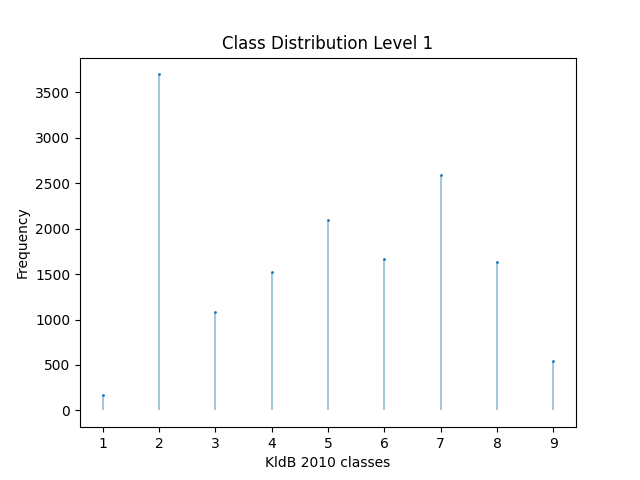
\includegraphics[width=.9\linewidth]{training_data_short_L1.png}
    \caption{\label{fig: F9} Class Distribution Level 1}
  \end{subfigure}%
  \begin{subfigure}{.5\textwidth}
    \centering
    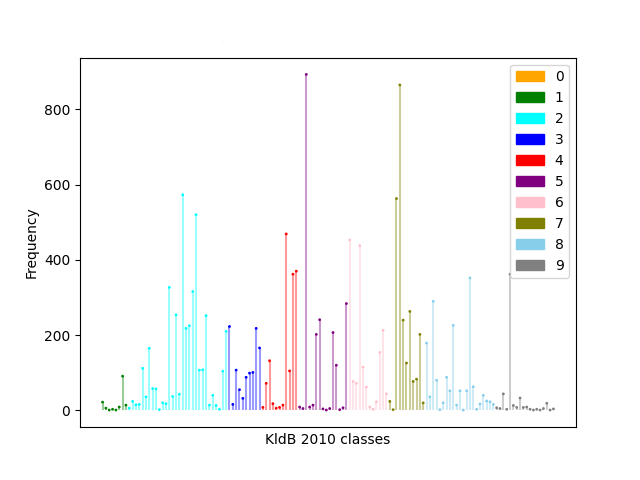
\includegraphics[width=.9\linewidth]{training_data_short_L3.png}
    \caption{\label{fig: F10} Class Distribution Level 3}
  \end{subfigure}
  \caption{Class Distribution of the Training Data}
  \end{figure}

Figures \ref{fig: F9} and \ref{fig: F10} show the distribution of the classes in level 1 and level 3.\footnote{The class distribution of the long dataset is given in the appendix.} Both figures show the absolute number of examples for each \textit{kldb} in the respective levels. In figure \ref{fig: F10} the number of examples is colored with the belonging \textit{kldb} level 1 class to give a better overview of the 144 \textit{kldbs} on level 3. In general, from both levels, it is clear that the data is not distributed equally. For the class distribution of level 1 on Figure \ref{fig: F9}, class 1 and class 9 have really few examples, while class 2 has considerably more examples than all other classes. Although the data is imbalanced, all classes have at least some examples to get meaningful performance measurements. At level 3, the uneven distribution is even more apparent. Compared to level 1, there are many classes with only one example, which is problematic for obtaining interpretable measurements. This issue will be discussed in the results section. Note that \textit{kldb} 0 is missing for level 1. Thus, it cannot be trained with the classifier. 0 stands for ``Militär". Jobs in this category are generally not posted frequently on the Employment Agency Job Board page, so it was not possible to get examples for this \textit{kldb}. On level 3 eight classes do not have any examples.


\section{Method}
\subsection{Overview of the Pipeline}
The classification process is divided into several steps. Figure \ref{fig: F8} gives an overview of the procedure. In the first step, the \ac{KldB} and the job title data are focused on the necessary variables. This is done by matching the \textit{kldb} ids from the \ac{KldB} dataset with the internal documentation id from the job title data. In the following steps, the targeted data is preprocessed. This preprocessed data is then transformed into numerical vectors. For this purpose, different vector representations are created using five vectorization techniques.

\begin{figure}[hb!]
  \center
  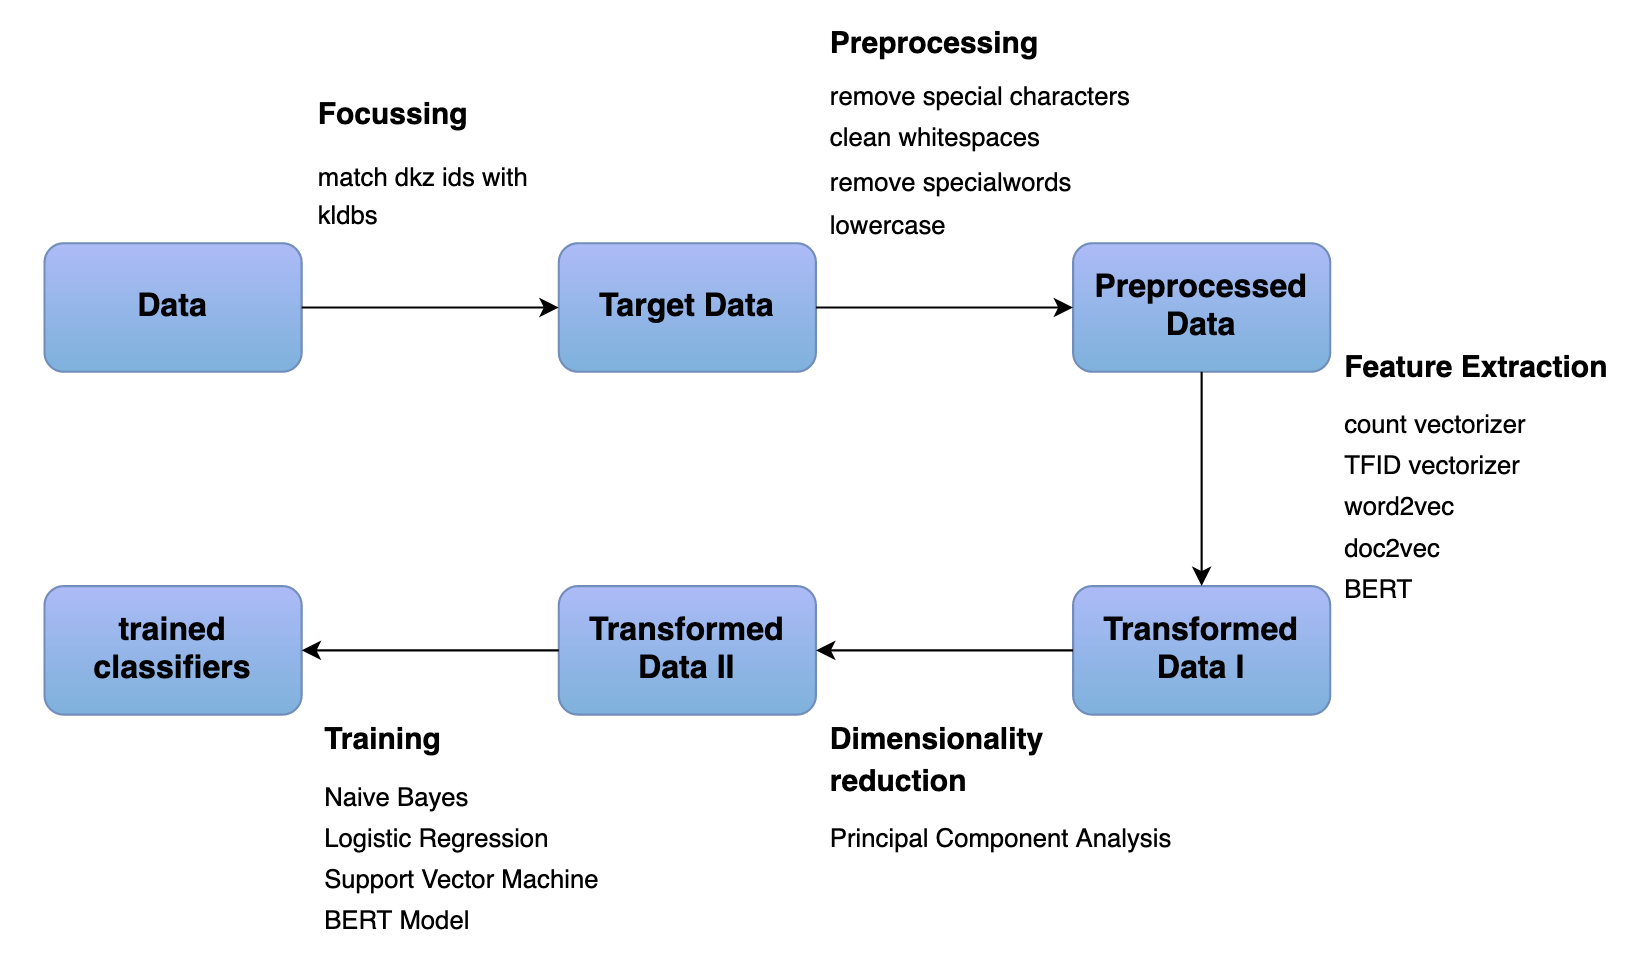
\includegraphics[scale=0.5]{pipeline_MA.png}
  \caption{\label{fig: F8} Training Pipeline}
\end{figure}

The transformed data is then reduced to lower dimensions using \ac{PCA}. The resulting data is the input for the classifier. In the last step, the four classifiers are trained. Note that the \ac{BERT} deep learning algorithm follows a different pipeline, which is why the algorithm is presented separately. Here, the data is put into the deep learning model directly after preprocessing, and the model is trained. The targeting of the data has already been described in the previous chapter. The remaining procedure and the associated methods are explained in detail in the following.\footnote{The code for this paper is publicly available at:

\url{https://github.com/Rahkakavee/job-title-matching.git}.} 

\subsection{Preprocessing}
Having an important influence on the performance of a classifier \citep{uysal2014, hacohen2020, gonccalves2005}, preprocessing is a crucial step that has to be taken before vectorization. There are several standardized practices for preprocessing like tokenization, stemming, stop word removal, and lowercasing \citep{alsmadi2019}. The methods of preprocessing used are justified below.

The first preprocessing step is removing special characters, which is necessary because most titles contain slashes and brackets to distinguish gender forms in occupational titles. Some job titles contain emojis, such as asterisks, which need to be removed because they are not related to specific job titles. 

Capitalized words are usually converted to lowercase to treat them equally for the classification. However, lowercase can be at the same time harmful for the performance if the interpretation changes with converting. The word `US", for example, which refers to the United States of America is equal to the pronoun ``us" if converted to lowercase. This can affect the performance if the differentiations play a role in the classification \citep{kowsari2019text}. Conversion makes sense for occupational names since capitalization plays a major role in German. In turn, I do not expect the conversion to cause problems often, as described in the example above, since occupational titles usually have specific names, and their lowercase variants do not often lead to other words or word classes. Thus, in a second step, titles are all converted to lowercase. 

As in every text classification task, stop word removal is a common praxis. All stop words, which are listed in the German stop words list of the Nature Language Toolkit package \citep{bird2009}, are removed. In addition, the data contained other peculiarities that justify the removal of other words besides stop words. Job titles often contain words, such as ``employee" or ``effective immediately", that do not contain important information and are not specific to particular job titles. In order to identify such words, the frequencies of each word across all documents are calculated. These frequencies are then used to identify words, such as ``employee", that are common but not relevant. As a final preprocessing step, the identified words are deleted from all job titles.  

\subsection{Vectorization Techniques}
\subsubsection*{Count Vectorizer}
The count vectorizer is one of the simplest methods for converting texts into vectors. It belongs to the family of \ac{BOW} models. \ac{BOW} models are based on vectors, where each dimension is a word from a vocabulary or corpus. The corpus is built by all words across all documents. \ac{BOW} models have two essential properties. Firstly, they do not consider the order of the words, sequences, or grammar. Secondly, each word in the corpus is represented by its own dimension. Thus, the vectors contain many zeros, especially for short texts, which is why they belong to the family of sparse vectors \citep{ajose2020}. Assuming that a corpus contains 1000 words, meaning each text is built only with these 1000 words, the vector for each text has a length of 1000, thus producing sparse, high-dimensional vectors \citep{kulkarni2021, sarkar2016}

The values for the vector are generated by counting for each text the frequency of the words occurring. Considering a corpus including only the three words ``java", ``developer" and ``python", the titles ``java developer" and ``python developer" would be encoded as follows:


\begin{table}[hb!]
\center
  \begin{tabular}{llll}
  \hline
                   & java & developer & python \\ \hline
  java developer   & 1    & 1         & 0      \\
  python developer & 0    & 1         & 1      \\ \hline
  \end{tabular}
  \caption{\label{tab: T11} Encoding with Count Vectorizer}
  \end{table}


As can be seen table \ref{tab: T11} results in the vectors $(1,1,0)$ and $(0,1,1)$. Note that if the title ``java developer" contains, for example, two times the word ``java", then the vector would change to (2,1,0). But since this is not a likely case for short text and especially job titles, the count vectorization here is for the most titles similar to one-hot vector encoding, which only considers the occurrence of the words, but not the frequency \citep{kulkarni2021, sarkar2016}

  While it is one of the most simple techniques, the count vectorizer has several limitations. The main downside is that it does not consider information like the semantic meaning of a text, the order, sequences, or the context. In other words, much information of the text is lost \citep{sarkar2016}. In addition, the count vectorizer does not consider the importance of words in terms of a higher weighting of rare words and a lower weighting of frequent words across all documents \citep{suleymanov2019}.

\subsubsection*{TF-IDF Vectorizer}
Like the count vectorizer \ac{TF-IDF} belongs to the family of \ac{BOW} and is a sparse vector as well. In contrast to the count vectorizer, it considers the importance of the words by using the \ac{IDF}. The main idea of \ac{TF-IDF} is to produce high values for words that often occur in documents but are rare over all documents. The \ac{TF} represents the frequency of a word t in a document d and is denoted by $tf(t,d)$. The \ac{DF}, denoted by $df$, quantifies the occurrence of a word over all documents. By taking the inverse of \ac{DF}, we get the \ac{IDF}. Intuitively, the \ac{IDF} should quantify how distinguishable a term is. If a term is frequent over all documents, it does not help distinguish between documents. Thus, the \ac{IDF} produces low values for common words and high values for rare terms and is calculated as follows \citep{sidorov2019, kuang2010}: 

\[idf(t) = log \frac{N}{df} \]

where N is the set of documents. The log is used to attenuate high frequencies. If a term occurs in every document, so $df = N$ the \ac{IDF} takes a value of 0 ($log (\frac{N}{N})$) and if a term is occuring only once in all existing documents, thus distinguishing perfectly from other documents, \ac{IDF} becomes 1 ($log (\frac{N}{1}$) \citep{sidorov2019}. Note that the calculation of \ac{IDF}s can be slightly adjusted \citep{robertson2004}. The implementation of sklearn package, which is used in this work, uses an adapted calculation \citep{scikit-learn}:

\[idf(t) = log \frac{1+n}{1+df(t)} + 1 \] 

Given the $idf(t)$ and $tf$ the \ac{TF-IDF} can be obtained by multiplying both metrics. In addition sklearn normalizes the resulting \ac{TF-IDF} vectors $v$ by the Euclidean norm \citep{scikit-learn}: 

\[v_{norm} = \frac{v}{||v||_2} \]

Although \ac{TF-IDF} considers the importance of words, as a \ac{BOW} model it suffers from the same limitation as the count vectorizer does by not taking semantic, grammatic, sequences, and context into account \citep{sarkar2016}. 

\subsubsection*{Word2vec}
In contrast to the sparse techniques mentioned above, word embedding techniques are another popular approach for vectorization. Word embedding vectors are characterized by low dimensions, dense representation, and continuous space. They are usually trained with neural networks \citep{li2015, jin2016}. 
  
Word2vec, introduced by \citet{mikolov2013}, is one computationally efficient word embedding implementation. The main idea of word2vec is based on the distributional hypothesis, which states that similar words often appear in similar context \citep{sahlgren2008}. Thus, word2vec learns with the help of the context representations of words, which include the semantic meaning and the context. In such a way, similar words are encoded similarly \citep{sarkar2016}. 

There exist two variants of word2vec. The first variant is based on \ac{BOW}, the so-called \ac{CBOW}, which predicts a word based on surrounding words. In contrast, the second variant, Skip-Gram, predicts the context words from a word \citep{ajose2020, sarkar2016}. This study uses a pre-trained model from Google, which is trained with \ac{CBOW}. Thus, in the following, the focus is on \ac{CBOW}. 

\begin{figure}[]
  \center
  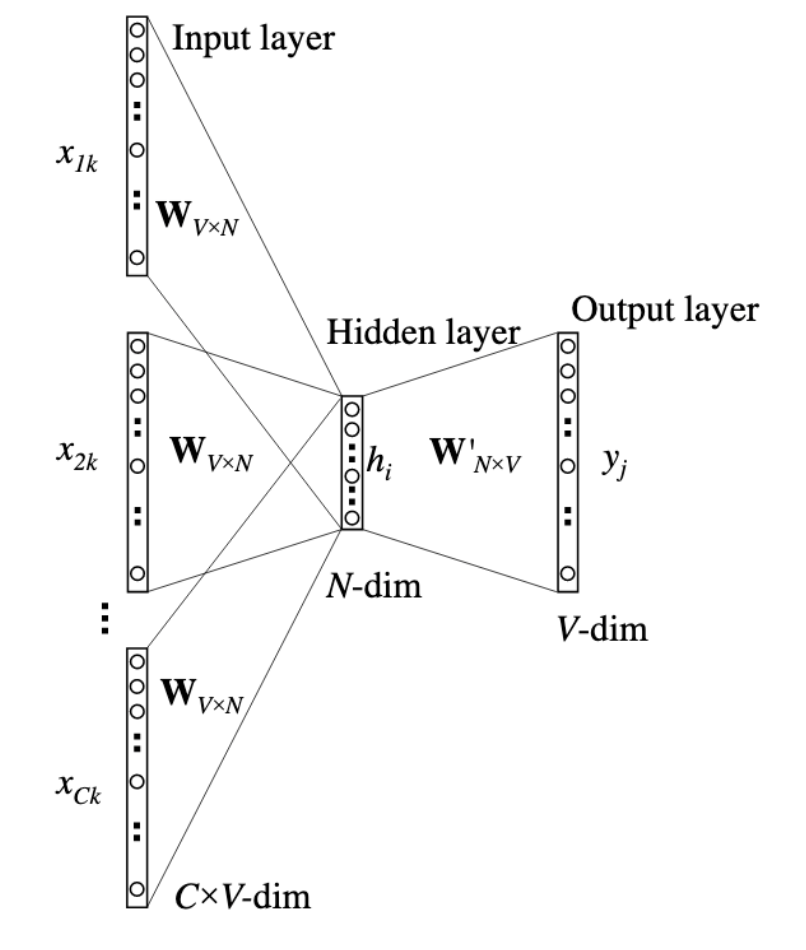
\includegraphics[scale=0.5]{word2vecCBOW.png}
  \caption[CBOW]{\label{fig: F1} CBOW \citep[6]{rong2014}}
\end{figure}

\ac{CBOW} word2vec is a 2-layer neural network with a hidden layer and an output softmax layer, which is visualized in figure \ref{fig: F1}. The goal is to predict a word, the so-called target word, by using the target word's context words. A certain window size defines the number of context words. If the window size is 2, the two words before and after the target word are considered. Given a vocabulary V, which is the unique set of words from the corpus, each context word c is fed into the neural network, encoded with a one-hot encoding of the length of V, building vector $x_c$. Thus, in figure \ref*{fig: F1} $x_{1k}$, for example, could be a one-hot encoded vector of the word before the target word. The weights between the input layer and the hidden layer are shown in figure \ref{fig: F1}. Taking the dimension of V and the hidden layer size N results in the $V \times N$ matrix W. Given that each row $v_w$ in W represents the weights of the associated word from the input and C equals the number of context words, the hidden layer h is calculated as follows \citep{rong2014}:

\[ h = \frac{1}{C} W^T(x_1 + x_2 + ... +x_c) = \frac{1}{C}(v_{w_1} + v_{w_2} + ... + v_{w_C}) \]

Since the context words are encoded with one-hot vector encoding, all except the respective word value in the vector, which is 1, will be 0. Thus, calculating h is just copying the k-th row of matrix W, thus an n-dimensional vector, which explains the second part of the equation. The hidden-layer matrix later builds the word embedding, which is why the decision on the size of the hidden layer later defines the dimensions for the word embedding vector \citep{rong2014}

From the hidden to the output layer, a $N \times V$ weight matrix is used to calculate scores for each word in V. A softmax function is used to get the word representation. Calculating the error and using backpropagation, the weights are updated respectively, resulting in a trained neural network. Due to computational efficiency, word2vec is trained with hierarchical softmax or negative sampling instead of the softmax function. Both methods are efficient because they reduce the amount of weight matrix updates \citep{rong2014, simonton2017}.\footnote{Since the focus is relying here on the word embeddings from the hidden layer and not the trained neural network itself, no further mathematical details will be given concerning the updating. For a detailed derivation see \citep{rong2014}}

Based on the given theoretical insights, I trained two word2vec models. Both models use a pre-trained model from Google and are fine-tuned with different data. The first model is fine-tuned with the complete dataset. The second model includes additional knowledge. The set-up is as follows: I use \ac{CBOW} word2vec models with a negative sampling technique. The hidden layer size and thus the word embedding vectors is 300, since the vectors have to have the same size as the pre-trained Google vectors. The minimal count of words is set to 1. The number of times the training dataset is iterated, the epoch number, is set to 10. Lastly, the window size for the context is set to 5. 

As the last step, the resulting word embeddings need to be processed in some way to get sentence embeddings for each job title. Word2vec cannot output sentence embeddings directly, which is why the word vector embeddings of each job title are averaged. 

\subsubsection*{Doc2vec}
Doc2vec, also known as paragraph vectors or Distributed Memory Model of Paragraph Vectors, is an extension method of word2vec, which outputs embeddings directly for each document \citep{lau2016}. It was proposed by \cite{le2014}. Doc2vec can be used for a variable length of paragraphs. Thus, it is applicable for more extensive documents, but also for short sentences like job titles \citep{le2014}. 

The main idea is, like for word2vec, to predict words in a paragraph. To do so a paragraph vector of that paragraph and word vectors are concatenated. The paragraph vector ``acts as memory that remembers what is missing from the current context - or the topic of the paragraph" \citep[3]{le2014}. Thereby, the paragraph vectors are trained with stochastic gradient descent and backpropagation. Similar to word2vec's practical implementation, doc2vec uses hierarchical softmax or negative sampling to speed up the training time \citep{lau2016}. 

\begin{figure}[]
  \center
  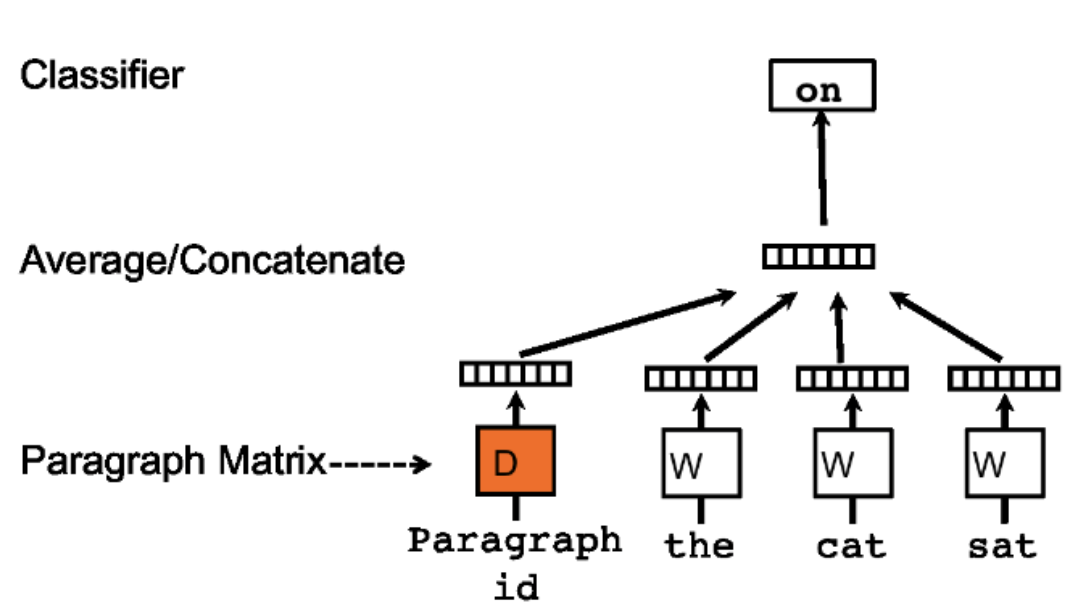
\includegraphics[scale=0.5]{doc2vec.png}
  \caption[Doc2vec - Distributed Memory Model of Paragraph Vectors]{\label{fig: F2} Doc2vec - Distributed Memory Model of Paragraph Vectors \citep[3]{le2014}}
\end{figure}

In figure \ref{fig: F2} the algorithm is visualized. The neural networks take word vectors and a paragraph vector as input. While the word vectors are shared over all paragraphs, each paragraph's paragraph vectors are unique. The paragraphs are represented as unique vectors in a column of a matrix D. The word vectors are expressed in the matrix W as before. In order to predict the word, both vectors are combined, for example, by averaging or concatenating. The doc2vec implementation described by \citet{le2014} and also used in this paper here concatenates the vectors. Formally, this only changes the calculation of h \citep{lau2016}. 

Since doc2vec is a word embedding method, it has the same advantages mentioned for word2vec. In addition, doc2vec takes the word order into account - at least in the same way a large n-gram would \citep{le2014}. Besides the model explained above, doc2vec also comes in a second variant, the so-called Distributed Bag of Words of Paragraph model, which ignores the word order. It is not clear which model performs better, although the inventor of doc2vec propose the first version \citep{lau2016}.

Based on this discussion, I created two Distributed Memory Models of Paragraph Vectors. Since there are no popular pre-trained models for doc2vec, I trained two custom models, one with the training data and one including the additional knowledge. I set the vector size to 300 with a window size of 5, a minimal count of 1, and trained ten epochs. Like word2vec, the models are trained with negative sampling. 

\subsubsection*{BERT}
\ac{BERT} uses a Multi-Layer Bidirectional Transformer Encoder as the architecture. This transformer architecture was established by \citet{vaswani2017}. It consists of an encoder and a decoder and makes use of self-attention. Both encoder and decoder stack include an identical layer. In addition, each of them includes two sub-layers: A multi-head attention and a feedforward network layer. It is out of the scope of this paper to elaborate on the technical details of the attention mechanism, which is why a simplified explanation is given. 

The self-attention mechanism improves the representation of a word, represented by a matrix X by relating it to all other words in the sentence. In the sentence ``A dog ate the food because it was hungry" \citep[10]{ravichandiran2021} the self-attention mechanism, for example, could identify that ``it" belongs to ``dog" and not to ``food" by relating the word to all other words. In order to compute the self-attention of a word, three additional matrices, the query matrix Q, the key matrix K, and a value matrix V are introduced. Those matrices are created by introducing weights for each of them and multiplying those weights with X. Based on those matrices, the dot product between the Q and the K matrix, a normalization and a softmax function is applied in order to calculate an attention matrix Z.\footnote{For a step-by-step calculating see \citep{ravichandiran2021}} \ac{BERT} uses a multi-head-attention, which means that multiple Z attention matrices instead of a single one are used.

\ac{BERT} takes one sentence or a pair of sentences as input. To do so, it uses a WordPiece tokenizer and three special embedding layers, the token, the segment, and the position embedding layer for each token, which is visualized in figure \ref{fig: F4}. A WordPiece tokenizes each word that exists in the vocabulary. If a word does not exist, words are split as long as a subword matches the vocabulary or an individual character is reached. Hashes indicate subwords. For the token embeddings, the sentence is tokenized first, then a [CLS] is added at the beginning of the sentence and a [SEP] token at the end. The job titles ``java developer" and ``python developer", for example, become tokens as shown in the token embedding row of figure  \ref{fig: F4}. In order to distinguish between the two titles, a segment embedding is added, indicating the sentences. Lastly, the \ac{BERT} model takes a position embedding layer, which indicates the order of the words. For each token, those layers are summed up to get the representation for each token \citep{devlin2018,ravichandiran2021}.

\begin{figure}[hb!]
  \center
  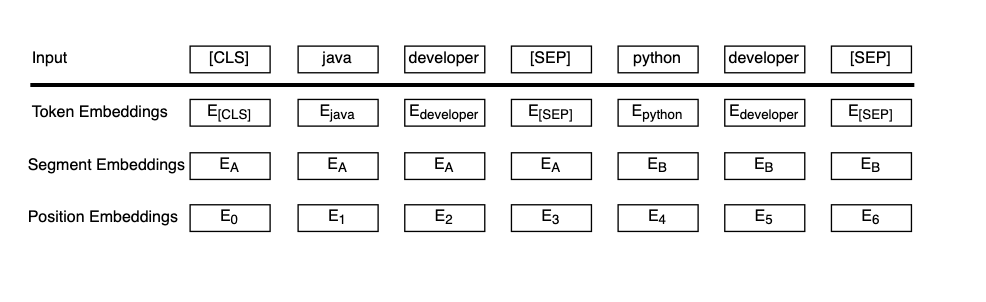
\includegraphics[scale=0.8]{BERTInput_own.png}
  \caption[Input of BERT]{\label{fig: F4} Input of BERT \citep[5]{devlin2018}}
\end{figure}

\begin{figure}[hb!]
  \center
  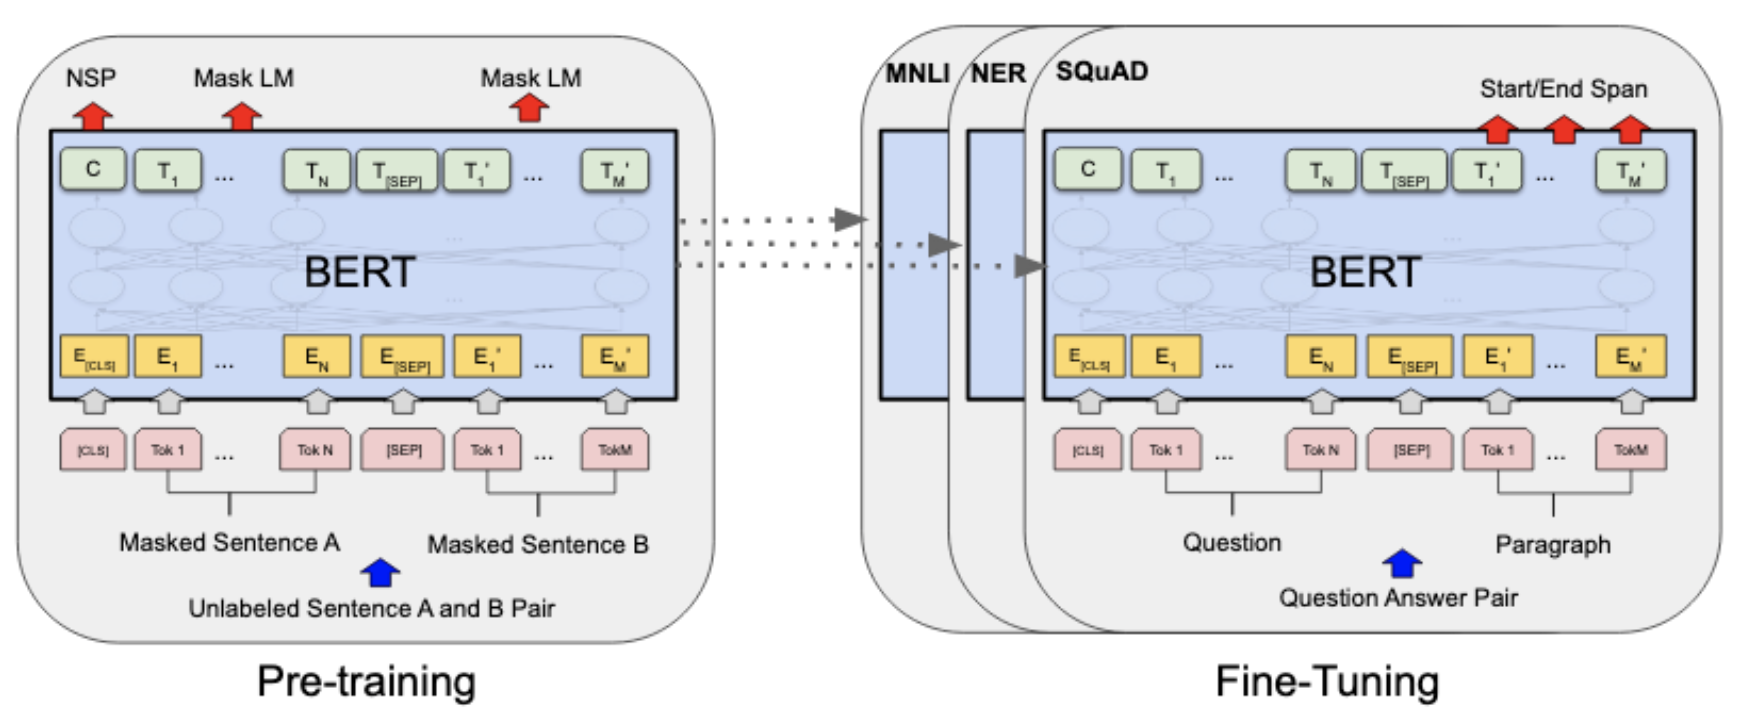
\includegraphics[scale=0.5]{BERTOverview.png}
  \caption[Overview BERT]{\label{fig: F3} Overview BERT \citep[3]{devlin2018}}
\end{figure}


The \ac{BERT} algorithm can be described in two steps. First, the pretraining phase, which is illustrated on the left-hand side of figure \ref{fig: F3} and the fine-tuning phase, which is visualized on the right-hand side. 

\paragraph{Pretraining}
The pretraining phase consists of two jobs: Masked language modeling and next sentence prediction. Masked language modeling means that a percentage of the input tokens are masked at random. For example, the job title ``python developer" could be masked as follows: [[CLS] python [MASK] [SEP]]. Since in fine-tuning tokens are not masked, a mismatch would occur between fine-tuning and pretraining, which is why not all of the masked tokens are matched with a [mask] token, but also with a random token or the real tokens.\footnote{There are specific rules of how to mask. See \citet{devlin2018} for detailed implementation} Instead of predicting the complete sentence, \ac{BERT} trains to predict the masked tokens. The prediction is performed with a feed-forward network and a softmax activation \citep{devlin2018,ravichandiran2021}. 

The second task retakes two sentences but predicts whether the first sentence is followed by the second one, which helps to understand the relationship between the sentences. Each sentence pair is labeled with either isNext or NotNext. By using the [CLS] token, which has the aggregating representation of all tokens, a classification task of whether a sentence pair is isNext or NotNext can be carried out \citep{ravichandiran2021,devlin2018}.

The pretraining of \ac{BERT} is, in contrast to the fine-tuning process, computationally expensive. There are plenty of pre-trained \ac{BERT} models for the German case, like ``bert-base-german-cased" or ``distilbert-base-german-cased".\footnote{All german \ac{BERT} models are open source and are accessible through the transformers library \citep{wolf2020}} In an evaluation of German pre-trained language models, \citet{assenmacher2021} conclude that the ``bert-base-german-dbmd-uncased" algorithm works quite well. Following their results and own tests on different models, "bert-base-german-dbmd-uncased`` and ``bert-base-german-cased" seem to have the best results, which is why they are used for the fine-tuning process. Both models consist of 12 encoder layers, 12 attention heads, and 768 hidden units, resulting in 110 million parameters. The first model was trained with 16GB of German texts, the second model with 12GB of German texts. 

\paragraph{Fine-Tuning}
The second phase, fine-tuning, can be performed differently, depending on the task. Either the weights of the pre-trained model are updated during the classification process, or the pre-trained model is first fine-tuned and then used as a feature extractor. 

I train two models with \ac{BERT}. While the first model includes a classification layer, in the following named \ac{BERT} deep learning model, the second model applies \ac{BERT} as a feature extraction method, in the following named \ac{BERT} vectorizer. 

The \ac{BERT} deep learning model is fine-tuned with the complete training dataset. Practically, this is done by converting the sentences of the dataset into the appropriate data format as described above and training it with the supervised dataset on some epochs, which then outputs the labels. From a theoretical point of view, the last hidden state of the [CLS] token with the aggregation of the whole sentence is used for the classification. In order to get the labels, \ac{BERT} uses a softmax function \citep{sun2019}. As already stated in the literature, it is not well-understood what exactly happens during the fine-tuning. An analysis of \citet{merchant2020} for other \ac{NLP} tasks than text classification indicates that the fine-tuning process is relatively conservative in the sense that they affect only a few layers and are specific for examples of a domain. The training set-up is as follows: Testing different epoch numbers indicates that smaller epoch size has better results for the model, which is why I fine-tune in 6 epochs. For the optimization, an adam algorithm, a gradient-based optimizer \citep{kingma2014}, with a learning rate of $1e^{-5}$ is used. 

In order to get sentence embeddings, different strategies, like averaging the output layer of \ac{BERT} or using the [CLS] token, are applied. Another method, developed by \citet{reimers2019} is sentence-\ac{BERT}, which is computationally efficient and practicable to implement. Since it facilitates encoding sentences directly into embeddings, I use it for the \ac{BERT} vectorizer. The model is constructed with the "bert-base-german-dbmd-uncased`` model and a pooling layer. The pooling layer is added to output the sentence embeddings. The fine-tuning process uses a siamese network architecture to update the weights. Figure \ref{fig: F5} shows the architecture. The network takes pairs of sentences with a score as an input. Higher scores indicate higher similarity between the sentences. The network updates the weights by passing the sentences through the network, calculating the cosine similarity, and comparing to the similarity score \citep{reimers2019}.

From the job title dataset and the \textit{kldb} dataset, I create pairs of similar and dissimilar job titles or search words. Similar pairs are pairs by being the same \textit{kldb} class. As a score, I choose 0.8. Dissimilar pairs are defined as pairs that are not from the same class. The score is 0.2. Building all combinations of titles and the search words for each class would result in a huge dataset. For example, class 1 of the training dataset has 2755 job titles, which results in ${2755 \choose 2} = 3793635$ pairs for class 1. Since this is computationally too expensive, I randomly choose pairs of job titles. For level 1, the following samples are drawn: From the job title data for each class, I used 3250 pairs. The same is true for the searchwords of each class. For unsimilar pairs, I used 1750 job title pairs, not from the same class. The same principle applies for the search words. This results in a total number of $(3250+3250) \times 9 + 2 \times 1750 = 62000$ pairs for the finetuning of level 1.\footnote{The determination of the exact number of pairs is exploratory, and runtime and performance were taken into account.} For level 3, the procedure is the same, only the numbers differ. For similar pairs of job titles and searchwords I used 400 for each class and for the unsimilar I used 6000 pairs. Classes with only one example are not considered because building pairs is impossible. This gives a total number of $(400 + 400) \times (136-7) + 2 \times 1500 =  61200$ pairs. 

\begin{figure}[hb!]
  \center
  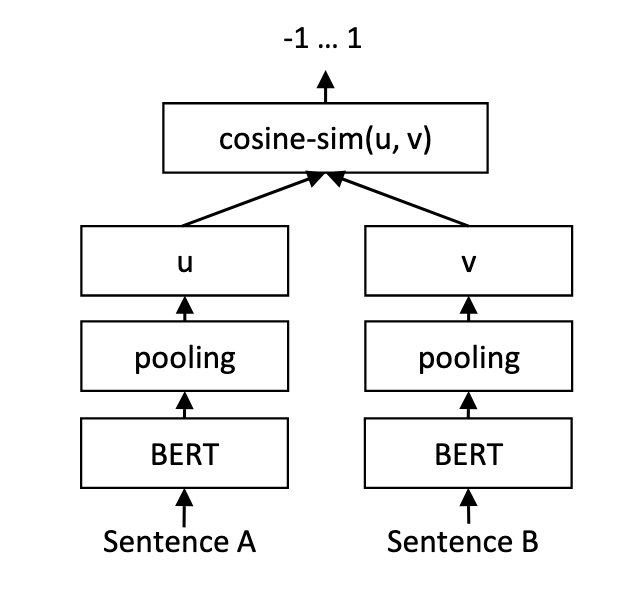
\includegraphics[scale=0.5]{SBERT.png}
  \caption[Sentence-BERT Siamese Structure]{\label{fig: F5} Sentence-\ac{BERT} Siamese Architecture \citep[3]{reimers2019}}
\end{figure}

\subsection{Dimensionality Reduction}
Dimensionality reduction techniques based for example on \ac{PCA} play an essential role in reducing computation time and saving computing resources \citep{ayesha2020}. Figure \ref{fig: F6} shows the runtime of all three classifiers with different data sizes and both with and without \ac{PCA}. 
\begin{figure}[]
  \center
  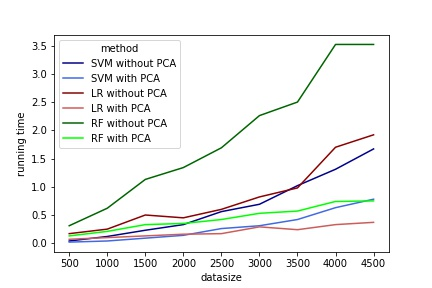
\includegraphics[scale=0.5]{running_time_PCA.jpeg}
  \caption{\label{fig: F6} Runtime of Word2vec with Different Data Sizes}
\end{figure}
The input for the classifiers are the word2vec embeddings without the additional knowledge. The bright lines show the runtimes without dimensionality reduction, while the dark-colored lines report the runtime with \ac{PCA} transformation. It becomes clear that the runtime for the transformed embeddings is generally lower. The magnitude of the differences is almost irrelevant for a dataset of 500. However, for the non-transformed embeddings, the runtime increases considerably with the dataset size for all classifiers. This is most evident with \ac{RF}. With increasing dataset size the runtime of the transformed embeddings also increases for all classifiers. However, it does so at a much slower pace. Therefore, it can be concluded that the transformation contributes to keeping the runtime lower for large datasets. As already described in chapter 3, the training dataset is pretty large, so it is reasonable to reduce the dimensions. 

\ac{PCA}, one of the most popular techniques for dimensionality reduction, aims to reduce a high-dimensional feature space to a lower subspace while capturing the essential information \citep{tipping1999, bisong2019}. The main idea is to use linear combinations of the original dimensions, so-called principal components, to reduce the dimensional space \citep{bro2014,geladi2017}.

Conceptually, the covariance matrix for the word embeddings is obtained in the first step. The covariance matrix, denoted by $\textbf{X}$, captures the linear relationships between the features of the word embeddings. In the next step, the eigenvectors of $\textbf{X}$ are calculated. The eigenvector of X is defined as \citep{bro2014}: 

\[ \textbf{X}z = \lambda z \]

where $z$ is the eigenvector and $\lambda$ the eigenvalue. In order to decompose $\textbf{X}$ to get the eigenvalue, Singular Value Decomposition is applied. The eigenvalues are sorted from highest to lowest, and the most significant components $n$ are kept. In order to choose $n$, the variance explained by the principal components is considered. The explained variance is set to $0.95$. In order to transform the data, a feature vector is generated. This vector contains the most $n$ significant eigenvalues. After transposing the mean-adjusted word embedding and the feature vector, the embeddings can be transformed by multiplying both transposed vectors \citep{smith2002}. 

\subsection{Classifiers}
In the following, based on a theoretical discussion of each classifier, the exact modeling is justified. The focus and depth of the explanations of the properties of the classifiers, such as decision function or regularization, depend on the settings chosen for the classification algorithms. Therefore, not all properties are described to the same extent for all classifiers. The \ac{BERT} deep learning model is already described in chapter 4.3. 

\subsubsection*{Logistic Regression}
\ac{LR}, a generalized linear model, is one of the most used analytical tools in social and natural science for exploring the relationships between features and categorical outcomes. For solving classification problems, it learns weights and a bias (intercept) from the input vector. Figure \ref{fig: F7} illustrates the idea of the calculation of \ac{LR}. To classify examples, first, the weighted sum of the input vector is calculated. For multi-classification, the weighted sum has to be calculated for each class. Thus, given a $f \times 1$ feature vector x with $[x_1, x_2, ..., x_f]$, a weight vector $w_k$ with $k$ indicating the class k of the set of classes K, a bias vector $b_k$, the weighted sum is defined as the dot product of $w_k$ and $\textbf{x}$ plus the $b_k$. Representing the weight vectors of each class in a $[K \times f]$ matrix $\textbf{W}$, the weighted sum can be formally expressed as $\textbf{W}x+b$. In Figure \ref{fig: F7}, the blue lines, for example, are a row in $\textbf{W}$ and the weight vectors are related to a class labeled with 1 \citep{jurafsky2021}.

\begin{figure}[hb!]
  \center
  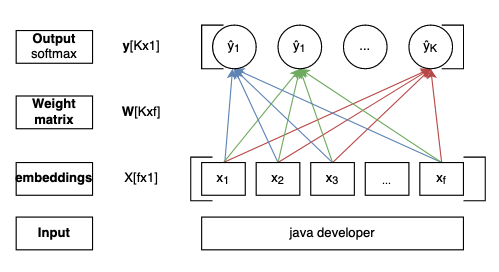
\includegraphics[scale=0.5]{LR.png}
  \caption[LR]{\label{fig: F7} MRL (edit after \citep[p.]{jurafsky2021})}
\end{figure}

In a second step, the weighted sums are mapped to a value range of $[0,1]$ to classify the input. While binary logistic regression uses a sigmoid function to do so, \ac{LR} with multiple classes needs a generalized sigmoid function. This generalization is called the softmax function, which outputs probabilities for each of the classes, which is why \ac{LR} is often called softmax regression in the literature. For each class $p(y_k = 1|x)$ is modeled. 

Similar to the sigmoid function, but applicable for multiple values, the softmax function maps each value of an input vector z with $[z_1, z_2, ..., z_K]$ to a value of the range of $[0,1]$. Thus, outputting a vector of length z and all values together summing up to 1. Formally it is defined as: 
\[ softmax(z_i) = \frac{exp(z_i)}{\sum^K_{j=1} exp(z_j)} \text{ } 1 \leq i \leq K \]

Then the output vector y can be calculated by: 

\[ \hat{y} = softmax(\textbf{W}x+b) \]

The goal of weight and bias training is to ``maximize the log probability of the true y labels" of the input data. This is commonly done by minimizing a generalized cross-entropy loss function for \ac{LR}. Different methods exist for solving the optimization problem, like stochastic gradient descent or limited-memory Broyden-Fletcher-Goldfarb Shannon solver. The latter converges rapidly and is characterized by a moderate memory, which is why it can converge faster for high-dimensional data \citep{fei2014, scikit-learn}. 

For \ac{LR} it is common to add a regularization parameter. This avoids overfitting and ensures that the model is more generalizable to unseen data. The idea is to penalize weights with good classification but using high weights more than weights with good classification but smaller weights. There are two popular penalty terms, the L1 and the L2 penalty. While for L1, the absolute values of the weights are summed and used as the penality term, L2 regularizes with a quadratic function of the weights. With the regularization, a parameter C is introduced to control the strength of the regularization. C is a positive value, and if smaller, it regularizes stronger \citep{jurafsky2021}. 

The following setting will be used for the \ac{LR}: A \ac{LR} with a L2 penalty with a C value of 1 is used. Since the input vectors, especially for count vectorizer and for \ac{TF-IDF} are high-dimensional, the limited-memory Broyden-Fletcher-Goldfarb-Shannon solver is set for solving. For some training, converge problems appeared, which is why the maximal iteration of the classifier is set to 10000.

\subsubsection*{Support Vector Machines}
 The general idea of a \ac{SVM} is to map ``the input vectors x into a high-dimensional feature space Z through some nonlinear mapping chosen a priori [...], where an optimal separating hyperplane is constructed'' \citep[138]{Vapnik2000}. This optimal hyperplane maximizes the margin, which is the distance from the hyperplane to the closest points, so-called Support Vectors, across both classes \citep{Han2012}. Formally, given a training dataset with n training vectors $x_i \in R^n, i = 1,....,n$ and the target classes $y_1,...y_i$ with $y_i \in \{-1, 1\}$, the following primal quadratic programming problem has to be solved in order to find the optimal hyperplane:
\[\min_{w,b} \frac{1}{2}w^{T}w \] 
\[\text{subject to } y_i(w^T\phi(x_i)+b) \geq 1\]

where $\phi(x_i)$ transforms $x_i$ into a higher dimensional space, $w$ corresponds to the weight and $b$ is the bias \citep{Chang2001,Jordan2006}.
The given optimization function assumes that the data can be separated without errors. Since this is not always possible, \cite{Cortes1995} has introduced a soft margin \ac{SVM}, which allows for misclassification \citep{Vapnik2000}.
By adding a regularization parameter $C$ with $C > 0$ and the corresponding slack-variable $\xi$ the optimization problem changes to \citep{Chang2001, Han2012}: 
\[\min_{w,b} \frac{1}{2}w^{T}w + C \sum_{i=1}^n \xi_i \] 
\[\text{subject to } y_i(w^T\phi(x_i)+b) \geq 1 - \xi_i, \] 
\[\xi_i \geq, i = 1,...,n\]

Introducing Lagrange multipliers $\alpha_i$ and converting the above optimization problem into a dual problem, the optimal $w$ satisfies \citep{Chang2001, Jordan2006}:
\[w = \sum_{I=1}^n y_i\alpha_i\phi(x_i)\]

with the decision function \citep{Chang2001}:
\[\text{sgn } (w^T\phi(x)+b) = sgn(\sum_{i=1}^n y_i \alpha K(x_i, x) +b)\]

$K(x_i, x)$ corresponds to a Kernel function, which allows calculating the dot product in the original input space without knowing the exact mapping into the higher space \citep{Han2012, Jordan2006}. 

In order to apply \ac{SVM} to multi-class problems, several approaches have been proposed. One strategy is to divide the multi-classification problem into several binary problems. A common approach here is the one-against-all method. In this method, as many \ac{SVM} classifiers are constructed as there are classes k. The k-th classifier assumes that the examples with the k label are positive labels, while all the other examples are treated as negative. Another popular approach is the one-against-one method. In this approach $k(k-1)/2$ classifiers are constructed, allowing to train the data of two classes within each classifier \citep{Hsu2002}. Besides, some researchers, like \citet{Crammer2001}, propose approaches that seek to solve the task in a single optimization problem.\footnote{For a detailed overview of all different methods and the method of \citet{Crammer2001} see \citet{Hsu2002,Crammer2001}}

In order to find a robust classifier, I checked \ac{SVM}s with different parameters, as well as different multi-class approaches. I found that a \ac{SVM} using a soft margin with a $C=1$ and a one-vs-rest approach yielded the best results. I also tested different kernels, like  RBF Kernel or linear kernel. The latter, formally  $k(x, x') = x^Tx'$ \citep{Jordan2006}, achieved the best results, which is why I chose it for the classifier. 

\subsubsection*{Random Forest Classifier}
In contrast to the previous two classifiers, \ac{RF} is an ensemble learning technique. The main idea of ensemble learning techniques is to create several learners and combine them. Those learners are, for example, a Decision Tree or neural networks and are usually homogeneous, meaning that each learner is based on the same machine learning algorithm. The different ensemble techniques are built on three pillars: the data sampling technique, the strategy of the training, and the combination method \citep{polikar2012, zhou2009}. 

The first pillar, data sampling, is important because it is not desirable to have the same outputs for all classifiers. Thus, ensemble techniques require diversity in the output, i.e. the outputs should be optimally independent and negatively correlated. Several methods for achieving diversity are already well established. Bagging techniques, for example, rely on bootstrap \citep{polikar2012}. The second pillar raises the question of which techniques should be applied to train the learners of the method. The most popular strategies for the training are bagging and boosting \citep{polikar2012}. The last pillar is about the combining method. Each classifier of the method will output an individual classification result, and those results have to be combined in some way to achieve an overall result. There are plenty of methods like majority voting or borda count \citep{polikar2012}.

\ac{RF} uses Decision Trees as its individual classifier. Before discussing \ac{RF} in more detail within the three pillars described above, a brief discussion of the Decision Tree is given in order to understand the mechanism and training procedure of the classifiers. 

The main idea of the Decision Tree algorithm is to ``break up a complex decision into a union of several simple decisions" \citep[660]{safavian1991} by using trees, with a root node on the top, intermediate nodes, and leaf nodes at the bottom. All possible splittings are checked and split according to the best feature for the root node and each intermediate node. Each leaf node leads to one of the classification labels. Examples are then classified by traversing the tree from top to bottom and choosing the branch that satisfies the attribute value for the example at each intermediate node. The construction of a Decision Tree is a recursive procedure \citep{Berthold2020, xia2008, cutler2012}. The algorithm stops for a specific node if all training set examples belong to the same class or if there are no features left for splitting. This might end in a tree with a high depth, which is why pruning is often applied to avoid overfitting \citep{Berthold2020}.


Regarding the construction of the tree, the type of splitting and the splitting criterion has to be discussed. There are mainly three types of splits: boolean splits, nominal splits, and continuous splits. The latter chooses a particular value from the continuous feature as the splitting value \citep{cutler2012, Berthold2020}. For example, considering a word embedding x with 300 dimensions and a node t of a Decision Tree, which is split into the nodes $t_{left}$ and $t_{right}$. The node t could have the split $x[209] <= 0.336$. Examples with a value smaller than or equal to $0.336$ at the dimension index $209$ of the embedding vector follow the branch to $t_{left}$, while all other examples follow the branch to $t_{right}$.

The splitting criterion is essential to identify the best feature for splitting. Intuitively, the criteria should split the data in such a way that leaf nodes are created quickly \citep{Berthold2020}. Several measurements can be applied to determine the best split for each node, like Gini Impurity or Information Gain. Since \ac{RF} uses Gini Impurity, only this criterion will be discussed in detail below. 

The gini value indicates the purity of a dataset D with n classes. It is defined as follows \citep[3156]{yuan2021}: 

\[Gini(D) = 1 - \sum_{i=1}^n p^2_i\]

where $p_i$ is the probability that a class n occurs in D. The more pure D is, the lower the value of the Gini value. In order to determine the best feature k, the dataset is partitioned based on feature k. For continuous features, as in word embeddings, this is done by a continuous split. Defining V as the total number of subsets and $D^v$ as one of the subsets, the Gini impurity for a feature k can be calculated as follows \cite{yuan2021}: 

\[\text{Gini index}(D,k) = \sum_{v=1}^V \frac{|D^v|}{|D|} Gini(D^v) \]

Conceptually the Gini Index is the weighted average of the Gini value for each subset of D based on a feature k. Thus, subsets with more samples are weighted more in the Gini index. The optimal feature $k^*$ is then determined by minimizing the Gini impurity overall features K \citep[3156]{yuan2021}: 

\[ k^* = arg \min_{k \in K} \text{Gini index} (D,k) \]

Based on the above theoretical explanations of the foundations of the Decision Tree, researchers have developed several algorithms to train Decision Trees, like Iterative Dichotomiser 3, C4.5, or \ac{CART}. Depending on the target \ac{CART} produces classification (for categorical variables) or regression trees (for numerical variables). It only construct binary trees. The algorithm uses Gini Index, and it can handle numerical and categorical input \citep{brijain2014}.

\ac{RF} belongs to the family of bagging ensemble techniques.
Bagging selects a single algorithm and trains several independent classifiers. The sampling technique is sampling with replacement (bootstrapping). Bagging combines the individual models by using either majority voting or averaging. \ac{RF} differs from the classic bagging method by also allowing the selection of a subset of features for each classifier from which the classifiers can select, rather than allowing them to select from the entire range of features. \citep{polikar2012, zhou2009, Berthold2020}. 

Formally \citet{breiman2001}, who introduced mainly the \ac{RF} algorithm, defines the classifier as follows:

\begin{quote}
``A random forest is a classifier consisting of a collection of tree-structured classifiers $\{h(\textbf{x}, \Theta_k), k = 1, ...\}$ where the ${\Theta_k}$ are independent identically distributed random vectors and each tree casts a unit vote for the most popular class at the input $\textbf{x}$." \citep[6]{breiman2001}. 
\end{quote}
$\Theta_k$ is a random vector created for each k-th tree. $\Theta_k$ must be independent of the vectors $\Theta_1...\Theta_{k-1}$ and thus of all random vectors of the previous classifiers. Nonetheless, the distribution of the random vectors remains. Combined with the training set, with $\textbf{x}$ as the input vector a classifier $h(\textbf{x}, \Theta_k)$ is constructed \citep{breiman2001}. The random component $\Theta_k$ is not explicitly used in practical implementation. Instead, it is rather used implicitly to generate two random strategies \citep{cutler2012}. The first strategy is bootstrapping, i.e. drawing a sample with replacement from the training dataset. In order to estimate the generalization error, the correlation and the variable importance, \citet{breiman2001} applied out-of-bag estimation. Out-of-bag estimation leaves out some portion of the training data in each bootstrap. The second strategy is to choose a random feature for the splitting. Thus, at each node from the set of features, only a subset is used to split. \ac{RF} does not apply pruning. The trees grow by applying \ac{CART}-algorithm. As combination method for classification \ac{RF} uses unweighted voting.\citep{cutler2012}.

Based on the above explanations, the implemented \ac{RF} has the following setting: The number of learners is 100. Gini is used as the splitting criterion. The maximal number of features is square root of the number of features. Note that sklearn, which is used to implement \ac{RF} here, uses an optimized algorithm of \ac{CART} \citep{scikit-learn}.

\section{Result}
\subsection{Evaluation Metrics}
Appropriate measurements are crucial for being able to meaningfully compare the performance of different algorithms \citep{Ferri2009}. There exist several metrics for the evaluation of classification approaches in the literature \citep{Fatourechi2008}. In the following, the selected metrics for performance measurement will be justified. 

Most metrics rely on a confusion matrix. For the multi-class case, this confusion matrix is defined as follows \citep{Kautz2017}: 
\begin{table}[]
  \center
  \begin{tabular}{lllll}
  \hline
            & Positive Examples      &           &             &             \\ \hline
  Positive Prediction  & $c_{1,1}$ & $c_{1,2}$ & $\dots$     & $c_{1,n}$   \\
            & $c_{2,1}$ & $c_{i,j}$ &             &             \\
            &  $\vdots$         &           & $\ddots$ &   $\vdots$\\
            & $c_{n,1}$ &           & $\dots$     & $c_{n,n}$   \\ \hline
  \end{tabular}
  \caption[Confusion Matrix]{\label{tab: T1} Confusion Matrix (adapted from \citep[113]{Kautz2017})}
  \end{table}


\FloatBarrier
Derived from the confusion matrix one can see that $c_{i, j}$ defines examples which belong to  \textit{class j} and are predicted as \textit{class i}. Based on the confusion matrix, the true positives of a current class $m$ can be defined as $tp_{m} = c_{m, m}$, i.e. examples correctly predicted as the current  \textit{class m}. The false negatives are defined as those examples which do not belong to the current \textit{class m}, but are predicted as k, formally written as $fn_{m} = \sum_{i=1, i \neq m}^n c_{i, m}$. Next, the true negatives are examples belonging to the current  \textit{class m}, but are not predicted as m. This can be represented through the formula $tn_{m} = \sum_{i=1, i\neq m}^n \sum_{j=1, j \neq m}^n c_{i,j}$. Last, false positives are defined as examples not belonging to  \textit{class m}, but are predicted as such. Formally this can be expressed as: $fp_{m} =  \sum_{i=1, i \neq m}^n c_{m, i}$ \citep{Kautz2017}

The \ac{OA} is one of the most common metrics for performance evaluation. It represents how well the classifier classifies across all classes correctly. Given that N is the number of examples, formally, the \ac{OA} can be expressed as: 
\[OA = \frac{\sum_{i=1}^m tp_i + tn_i}{N} \]

An accuracy of 1 means that all examples are correctly classified. 0 means that each example is classified with the wrong class \citep{Berthold2020}. Although \ac{OA} is a widely used metric, it is criticized for favoring the majority classes and therefore not adequatley reflecting minority classes in unbalanced datasets \citep{Berthold2020, Fatourechi2008}.

Two more popular metrics are precision and recall. Precision represents how well the classifier detects actual positive examples among the positive predicted examples. Recall, also called sensitivity, in contrast, represents how many examples are labeled as positive among the actual positive examples \citep{Berthold2020}. For the multi-class scenario, two different calculation approaches for each of the metrics are proposed: micro and macro average. In the macro approach the metric for each \textit{class m} is first calculated against all other classes. Then, the average of all of them is computed. Given that $K$ is the total number of classes the macro precision and recall are calculated as \citep{Branco2017}:

\[precision_{macro} = \frac{1}{M} \sum_{i=1}^m \frac{tp_{i}}{tp_{i} + fp_{i}}\]
\[recall_{macro} = \frac{1}{M} \sum_{i=1}^m \frac{tp_{i}}{tp_{i} + fn_{i}}\]

In contrast to the macro apporach, the micro approach aggregates the values, which can be formally expressed as follows \citep{Branco2017}: 

\[precision_{micro} = \frac{\sum_{i=1}^m tp_i}{\sum_{i=1}^m tp_i + fp_i}\]
\[recall_{micro} = \frac{\sum_{i=1}^m tp_i}{\sum_{i=1}^m tp_i + fn_i}\]

There is a trade-off between precision and recall \citep{Buckland1994}. The F-score captures precision and recall by taking the harmonic mean between the two. It is calculated as follows \citep{Branco2017,Pan2016}:  

\[F_{micro} = 2 \cdot \frac{precision_{micro} \cdot recall_{micro} }{precision_{micro} + recall_{micro} }\ \]

\[F_{macro} = 2 \cdot \frac{precision_{macro} \cdot recall_{macro} }{precision_{macro} + recall_{macro} }\ \]

A closer look at the formula of the micro scores shows that actually, the micro precision and recall score are the same since aggregating the false negatives and aggregating the false positive results in the same number. If the precision and recall are the same, it follows from the F1-score calculation that it has to be equal as well. And even further, the micro score is actually equal to the accuracy. Thus the micro score suffers from the same problem as accuracy \citep{grandini2020}.

Since the job title classification involves multi-class classification and the descriptive analysis has shown that the data is imbalanced, it is not reasonable to base the evaluation solely on the \ac{OA}. Showing that micro scores are all equal, it is crucial to take the macro scores into account to capture the performance of the minority classes well.

\subsection{Experimental Results}
As explained above, the results are compared from three perspectives: Vectorization techniques, classification algorithms, and enrichment with additional knowledge. Table \ref{tab: T5} and \ref{tab: T6} show the results of level 1 for all vectorization methods. Each row denotes a vectorization technique. Each column represents a classifier. Table \ref{tab: T5} reports the accuracy while table \ref{tab: T6} reports the macro precision (p), recall( r) and F1-score (F1). Word2vec and doc2vec without additional knowledge training are marked with $I$, the ones with additional knowledge by $II$. The results of the \ac{BERT} deep learning model are reported separately in table \ref{tab: T12}. 


\begin{table}[hb!]
  \center
\begin{tabular}{lrrr} 
  \hline
  {} &    \textbf{LR} &   \textbf{SVM} &    \textbf{RF} \\
  \hline
Count Vectorizer &  0.72 &  0.69 &  0.65 \\
TF-IDF           &  0.72 &  0.69 &  0.65 \\
Word2vec\_I      &  0.54 &  0.53 &  0.61 \\
Word2vec\_II     &  0.54 &  0.52 &  0.62 \\
Doc2vec\_I       &  0.48 &  0.46 &  0.56 \\
Doc2vec\_II      &  0.45 &  0.42 &  0.53 \\
BERT            &  0.78 &  0.78 &  0.77 \\
  \hline
  \end{tabular}
  \caption{\label{tab: T5} Evaluation of Level 1 Classification - Accuracy}
\end{table}


\begin{table}[]
    \resizebox{\textwidth}{!}{%
  \begin{tabular}{llll}
  \hline
  {} &                          \textbf{LR} &                         \textbf{SVM} &                          \textbf{RF} \\
  \hline
  Count Vectorizer &  p: 0.76, r: 0.61, F1: 0.66 &  p: 0.72, r: 0.58, F1: 0.63 &  p: 0.66, r: 0.53, F1: 0.57 \\
  TF-IDF           &  p: 0.77, r: 0.61, F1: 0.65 &  p: 0.73, r: 0.58, F1: 0.62 &  p: 0.67, r: 0.53, F1: 0.57 \\
  Word2vec\_I      &  p: 0.58, r: 0.39, F1: 0.42 &   p: 0.46, r: 0.40, F1: 0.41 &  p: 0.58, r: 0.52, F1: 0.54 \\
  Word2vec\_II     &  p: 0.59, r: 0.41, F1: 0.45 &  p: 0.48, r: 0.41, F1: 0.43 &  p: 0.59, r: 0.53, F1: 0.55 \\
  Doc2vec\_I       &  p: 0.51, r: 0.33, F1: 0.35 &  p: 0.41, r: 0.33, F1: 0.34 &   p: 0.59, r: 0.40, F1: 0.43 \\
  Doc2vec\_II      &   p: 0.54, r: 0.30, F1: 0.32 &   p: 0.37, r: 0.30, F1: 0.31 &   p: 0.55, r: 0.38, F1: 0.40 \\
  BERT            &  p: 0.76, r: 0.76, F1: 0.76 &  p: 0.75, r: 0.77, F1: 0.76 &  p: 0.78, r: 0.72, F1: 0.74 \\
  \hline
  \end{tabular}
    }
  \caption{\label{tab: T6} Evaluation of Level 1 Classification - Macro}
  \end{table}


\begin{table}[]
  \resizebox{\textwidth}{!}{%
  \begin{tabular}{llllllll}
  \hline
   &
    \textbf{Accuracy} &
    \textbf{Precision Macro} &
    \textbf{Recall Macro} &
    \textbf{F1 Macro} & \\ \hline
  \textbf{BERT Clf Level 1} &
    0.76 &
    0.71 &
    0.71 &
    0.71 & \\
  \textbf{BERT Clf Level 3} &
    0.44 &
    0.20 &
    0.18 &
    0.17 &\\ \hline
  \end{tabular}
  }
  \caption{\label{tab: T12} Evaluation of Level 1 and 3 BERT Deep Learning Model}
  \end{table}

Comparing the accuracy of the vectorization techniques, with approx. $78\%$ accuracy the \ac{BERT} vectorizer outperforms the other methods. A look at the macro table \ref{tab: T6} for \ac{BERT} confirms the high performance with relatively similar macro scores over all classifiers. Only in combination with \ac{RF}, the recall and thus the F1-score is lower with \ac{BERT} compared to the other classifiers. Further, the two sparse techniques count vectorizer and \ac{TF-IDF} performed quite well, especially compared to the word embedding techniques word2vec and doc2vec regardless of having additional knowledge or not for \ac{LR} and \ac{SVM}. Related to \ac{LR} and \ac{SVM}, the worst performance is achieved by doc2vec. However, word2vec also performs considerably below the sparse vectors and \ac{BERT}. For example, word2vec\_I has $18\%$ less accuracy than the count vectorizer for \ac{LR}. This picture is confirmed when looking at the macro table. The difference between word2vec and doc2vec on one side compared to the sparse vectors and the \ac{BERT} vectorizer on the other side shows up more strongly. Again for \ac{LR}, in comparison with word2vec\_I, the count vectorizer performed $24\%$ better, measured by the F1-score. 

A different picture is given for \ac{RF}. The differences between the sparse methods and the word2vec techniques is much smaller and for the macro scores almost vanished, while doc2vec performs lower. Finally, compared to \ac{BERT} vectorizer, all other vectorizers are performing lower, taking the macro score as a performance metric instead of accuracy. Note that doc2vec has ill-defined scores for \ac{LR} and \ac{RF} and word2vec for \ac{SVM} since they have no predictions for some classes. Considering the formula of the macro score above, if a class has zero examples, this class is set to zero but is included in the average. Hence, the macro scores for these vectorization techniques combined with the respective classifiers must be interpreted with caution. 

The analysis of the classification algorithms confirms the vague impression in the literature. While \ac{LR} and \ac{SVM} have an excellent performance for the dense vectorization techniques, \ac{RF} shows the best performance for the two word embedding techniques word2vec and doc2vec. For \ac{BERT}, on the other hand, all classification algorithms turn out to be strong. The \ac{BERT} deep learning model performed lower than the \ac{BERT} vectorizer but better than the other vectorization techniques. 

Concerning the last analysis dimension, the focus relies on word2vec\_II and doc2vec\_II, which contain additional knowledge for the embeddings.\footnote{The \ac{BERT} model contains as well additional knowledge since search words pairs also were used for the fine-tuning. However, the model comparison is difficult since \ac{BERT} deep learning model was trained differently and allows no direct comparison.} The accuracy score in table \ref{tab: T6}  of word2vec\_II shows no improvement by adding knowledge. For doc2vec, the results are even slightly worse, which is also reflected in the macro results. The macro results for word2vec show slightly better performance adding knowledge for \ac{SVM} and \ac{LR}, but for \ac{RF} this improvement has almost disappeared.

Table \ref{tab: T8} and \ref{tab: T10} contain the results of level 3. Again the results of the \ac{BERT} deep learning model are reported separately in \ref{tab: T12}. A problem is that many classes only have one example. Thus, there are often zero predictions for many classes overall classifiers and vectorization methods. This leads to ill-defined macro scores. At the same time, the accuracy still suffers from the mentioned problems of favoring classes. Nevertheless, the performance of the classifiers can be compared, since all suffer more or less equally from the classes without predictions. However, not too much meaning should be given to the exact percentages.

\begin{table}[hb!]
  \center
\begin{tabular}{lrrr}
\hline
{} &   \textbf{LR} &   \textbf{SVM} &    \textbf{RF} \\
\hline
Count Vectorizer &  0.50 &  0.52 &  0.44 \\
TF-IDF           &  0.48 &  0.53 &  0.45 \\
Word2vec\_I      &  0.30 &  0.15 &  0.36 \\
Word2vec\_II     &  0.30 &  0.20 &  0.35 \\
Doc2vec\_I       &  0.19 &  0.19 &  0.30 \\
Doc2vec\_II      &  0.16 &  0.16 &  0.27 \\
BERT            &  0.50 &  0.46 &  0.45 \\
\hline
\end{tabular}
\caption{\label{tab: T8} Evaluation of Level 3 Classification - Accuracy}
\end{table}


\begin{table}[hb!]
  \resizebox{\textwidth}{!}{%
\begin{tabular}{llll}
\hline
{} &                          \textbf{LR} &                         \textbf{SVM} &                          \textbf{RF} \\
\hline
Count Vectorizer &   p: 0.41, r: 0.27, F1: 0.30 &   p: 0.40, r: 0.34, F1: 0.35 &  p: 0.36, r: 0.25, F1: 0.28 \\
TF-IDF           &   p: 0.40, r: 0.23, F1: 0.27 &  p: 0.39, r: 0.33, F1: 0.35 &  p: 0.39, r: 0.26, F1: 0.29 \\
Word2vec\_I      &  p: 0.18, r: 0.12, F1: 0.12 &  p: 0.08, r: 0.06, F1: 0.05 &   p: 0.24, r: 0.19, F1: 0.20 \\
Word2vec\_II     &  p: 0.25, r: 0.14, F1: 0.17 &   p: 0.13, r: 0.11, F1: 0.10 &   p: 0.27, r: 0.20, F1: 0.22 \\
Doc2vec\_I       &  p: 0.11, r: 0.05, F1: 0.05 &  p: 0.12, r: 0.09, F1: 0.09 &  p: 0.22, r: 0.13, F1: 0.14 \\
Doc2vec\_II      &  p: 0.09, r: 0.04, F1: 0.04 &  p: 0.11, r: 0.07, F1: 0.08 &  p: 0.19, r: 0.11, F1: 0.12 \\
BERT            &  p: 0.58, r: 0.51, F1: 0.53 &  p: 0.52, r: 0.48, F1: 0.48 &  p: 0.48, r: 0.33, F1: 0.36 \\
\hline
\end{tabular}
}
\caption{\label{tab: T10} Evaluation of Level 3 Classification - Macro}
\end{table}

In general, the performance of level 3 is lower than level 1, which is due to the higher number of classes and lower number of examples in the classes. In contrast to level 1, there is no noticeable difference in accuracy between \ac{BERT} and the sparse vectors. However, looking at the macro scores, \ac{BERT} has a much higher recall, and thus a higher F1-score than the other techniques. In general, while the macro results for all other techniques reveal much worse performance compared to the accuracy score, \ac{BERT} is stable overall metrics. Thus, again it can be concluded that \ac{BERT} outperforms the other classifiers. Both sparse vectors performed relative equally. Comparing the sparse vectors against the word embeddings word2vec and doc2vec, the latter are the inferior. Same as for level 1, doc2vec has the worst performance.

Comparing the classifiers for level 3 shows the same picture for sparse vectors and word embeddings. Sparse vectors and \ac{BERT} vectorizer perform better with \ac{LR} and \ac{SVM}, while the word embeddings have the best result with \ac{RF}. In contrast to level 1, the best performance for \ac{BERT} is achieved by \ac{LR} on level 3, especially compared to the deep learning model, which performed much lower than the \ac{BERT} vectorization and looking at the macro results even much worse than the sparse techniques. However, concerning the results of \ac{BERT} of \ac{LR} and \ac{SVM}, a peculiarity should be noted. During training, there was no convergence of \ac{SVM} with \ac{BERT} in a real runtime. Therefore, a maximal iteration of $10000$ was set. This might have affected the performance of \ac{SVM}. Thus, one should be careful to rank \ac{LR} as considerably better than \ac{SVM}. 

Including additional knowledge in word2vec reveals no noticeable improvement for \ac{LR} and \ac{RF}. For \ac{SVM}, there seems to be slightly better results. The trend of macro results across all classifiers seems to confirm an improvement, although, for \ac{RF}, the enhancement is not too great and should not be given too much attention due to the ill-defined scores. The same problem applies to doc2vec. Roughly compared, there is no difference between doc2vec\_I and doc2vec\_II. However, the somewhat poorer performance of doc2vec\_II becomes apparent with some classification algorithms. 


\subsection{Deep Dive into the Results}
Looking at the results, we see some trends emerging. Comparing the vectorization techniques in both level 1 and level 3, the \ac{BERT} vectorizer has the best performance. The sparse ones perform better than the embedding techniques word2vec and doc2vec for \ac{LR} and \ac{SVM}, while there is little difference for \ac{RF}. Doc2vec performs the worst in general. Concerning the classifiers, \ac{RF} has lower performance overall but a better performance for word2vec and doc2vec compared to their results for \ac{LR} and \ac{RF}. While the deep learning model for level 1 has a comparable but lower performance than \ac{BERT} vectorization, it slips down to the performance of sparse vectors at level 3. Finally, the additional knowledge seems to lead to slightly better results for word2vec except for \ac{RF} for level 1. Doc2vec, in contrast, often shows slightly better results without adding the knowledge. Another noticeable result is that macro results are often worse than the accuracy implied, except for the \ac{BERT} vectorizer. All these trends require explanation. To get a better insight into the black box of the classifiers and the vectorization techniques, it is helpful to look at the actual predictions of the classifiers.

\subsection*{Possible Explanations for Level 1 Results}
For this purpose, the predictions of the test dataset are used. In the first step, the predictions for all methods and classifiers are obtained. Then the distribution of the class labels is analyzed to find possible patterns. The left-hand side of figure \ref{fig: F13} shows the share of prediction labels of \ac{LR} for all vectorization techniques except the ones with additional knowledge. For all methods, class 2 exhibit the highest prediction shares. 
Interestingly, the share of the two embedding techniques, word2vec and docv2vec, is about the same but much higher than for other methods. Likewise, the sparse vectors form a group and have a substantially higher share than \ac{BERT}. If we look at the proportions of \ac{BERT}, the labels are more evenly distributed. There are two possible explanations for this. Either class 2 is represented in a high proportion in the test dataset, and word2vec and doc2vec have led to better recognition, or the classifiers are more or less biased towards class 2, depending on the method. The class distribution in Figure \ref{fig: F9} shows that the data is imbalanced in favor of class 2. In addition the macro scores, which capture the imbalanced data better, are lower for most models . Thus, it is likely that the classifiers are biased. 

\begin{figure}[hb!]
  \centering
  \begin{subfigure}[b]{0.475\textwidth}
      \centering
      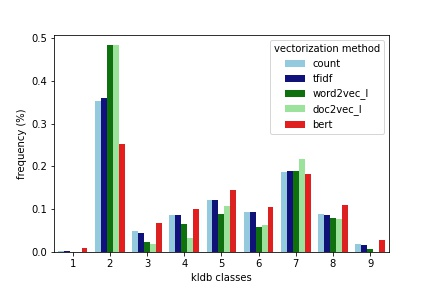
\includegraphics[width=\textwidth]{predictions_LR.jpg}
      { \bigskip
        {\small Share of Predictions Labels for Level 1 - LR}
      }    
  \end{subfigure}
  \hfill
  \begin{subfigure}[b]{0.475\textwidth}  
      \centering 
      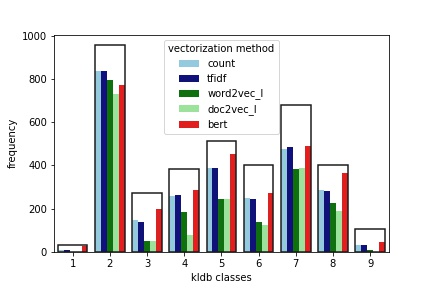
\includegraphics[width=\textwidth]{predictions_correct_relative_LR.jpg}
      {{\small Frequency of Correct Predictions for each Labels and Frequency of True Labels - LR}}    
  \end{subfigure}
\caption{\label{fig: F13} Predictions Level 1- LR}
\end{figure}

\begin{figure}[hb!]
  \centering
  \begin{subfigure}[b]{0.475\textwidth}
      \centering
      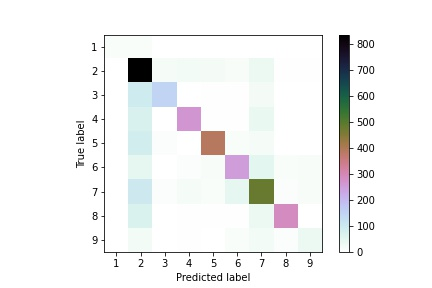
\includegraphics[width=\textwidth]{cm_count_LR.jpg}
      {{\small Count Vectorizer }}    
  \end{subfigure}
  \hfill
  \begin{subfigure}[b]{0.475\textwidth}  
      \centering 
      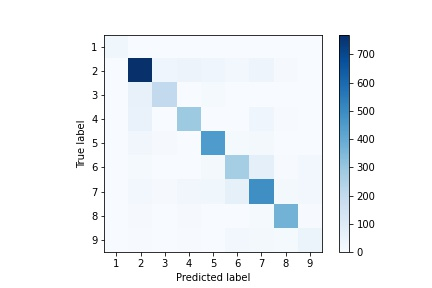
\includegraphics[width=\textwidth]{cm_bert_LR.jpg}
      {{\small \ac{BERT}}}    
  \end{subfigure}
  \vskip\baselineskip
  \begin{subfigure}[b]{0.475\textwidth}   
    \centering 
    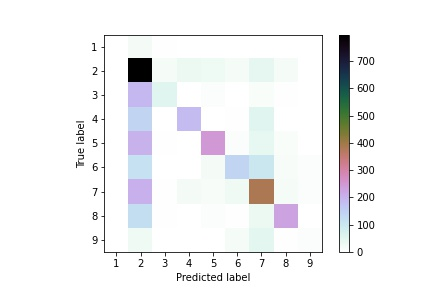
\includegraphics[width=\textwidth]{cm_word2vec_without_LR.jpg}
    {{\small Word2vec\_I}}    
  \end{subfigure}
  \hfill
  \begin{subfigure}[b]{0.475\textwidth}   
      \centering 
      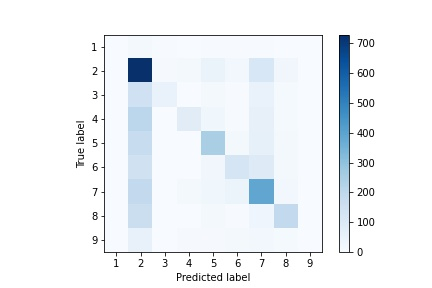
\includegraphics[width=\textwidth]{cm_doc2vec_without_LR.jpg}
      {{\small Doc2vec\_I}}    
  \end{subfigure}
  \caption{\label{fig: F17} Confusion Matrices - LR}
\end{figure}

To shed light on this issue, one can look at the correct predictions. The right-hand side of figure \ref{fig: F13} shows the correct predictions for each method for \ac{LR}, as well as the number of true labels for each class. At first glance, it looks like the classifiers predicted class 2 very well, especially compared to \ac{BERT}. However, for the other labels, the two embedding techniques, doc2vec and word2vec, have a much worse performance than the other methods, indicating a bias. The situation is similar for the sparse vectors compared to \ac{BERT}. Obviously, the excellent performance for class 2 is not due to the good differentiation of class 2, but to the fact that simply a very high proportion of predictions lay in class 2. 

To add further evidence for the presence of the bias, it is interesting to look at the predictions of class label 2 in comparison to the true labels. For this purpose, the confusion matrix as explained in the matrix \ref{tab: T1} can be considered. Figure \ref{fig: F17} shows the confusion matrices for all methods without additional knowledge. Also, \ac{TF-IDF} is left out because the sparse vectors behave relatively similarly. Thus, it is enough to check one of the techniques.\footnote{For the sake of completeness, the \ac{TF-IDF} confusion matrices are included in the appendix.} The x-axis represents the predicted labels, and the y-axis the actual labels. For doc2vec and word2vec, a vertical line is visible at the predicted label 2. This line shows that both methods often classified labels as 2, although they belong to one of the other labels. At the same time, they did not do so for the other labels. For doc2vec, this vertical line is even more apparent. The count vectorizer also has a stronger vertical line compared to \ac{BERT}, while \ac{BERT} seems to have treated all labels equally. Figure \ref{fig: F17} thus again provides strong evidence for the bias.\footnote{Detecting a labeling bias for a classification algorithm requires systematic analysis, as proposed by \citet{jiang2020}. Since this is beyond the scope of this paper, the confusion matrix, which gives a good indication of whether a possible bias exists,
is used here.}

\begin{figure}[hb!]
  \centering
  \begin{subfigure}[b]{0.475\textwidth}
      \centering
      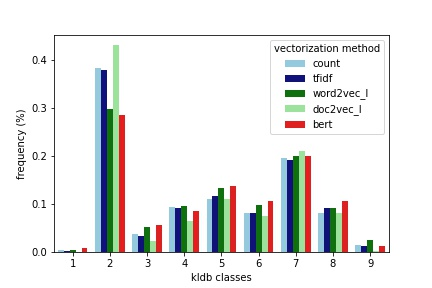
\includegraphics[width=\textwidth]{predictions_RF.jpg}
      {
        {\bigskip
          \small Share of predictions labels for level 1 - RF}
      }    
  \end{subfigure}
  \hfill
  \begin{subfigure}[b]{0.475\textwidth}  
      \centering 
      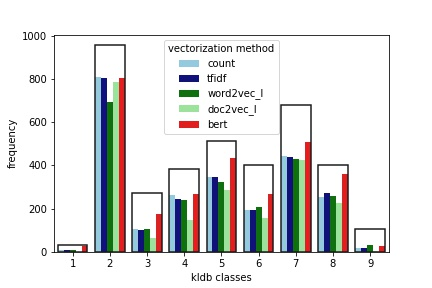
\includegraphics[width=\textwidth]{predictions_correct_relative_RF.jpg}
      {{\small Frequency of correct predictions for each labels and frequency of true labels - \ac{RF}}}    
  \end{subfigure}
\caption{\label{fig: F18} Predictions Level 1- RF}
\end{figure}


\begin{figure}[hb!]
  \centering
  \begin{subfigure}[b]{0.475\textwidth}
      \centering
      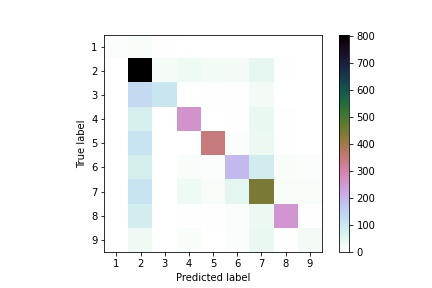
\includegraphics[width=\textwidth]{cm_count_RF.jpg}
      {{\small Count Vectorizer }}    
  \end{subfigure}
  \hfill
  \begin{subfigure}[b]{0.475\textwidth}  
      \centering 
      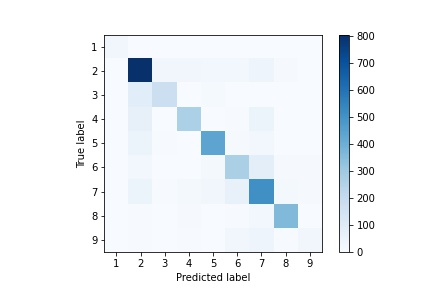
\includegraphics[width=\textwidth]{cm_bert_RF.jpg}
      {{\small \ac{BERT}}}    
  \end{subfigure}
  \vskip\baselineskip
  \begin{subfigure}[b]{0.475\textwidth}   
    \centering 
    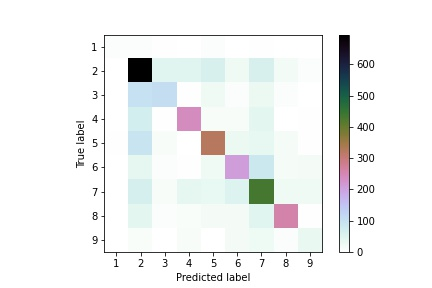
\includegraphics[width=\textwidth]{cm_word2vec_without_RF.jpg}
    {{\small Word2vec\_I}}    
  \end{subfigure}
  \hfill
  \begin{subfigure}[b]{0.475\textwidth}   
      \centering 
      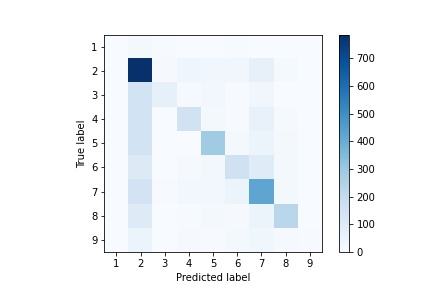
\includegraphics[width=\textwidth]{cm_doc2vec_without_RF.jpg}
      {{\small Doc2vec\_I}}    
  \end{subfigure}
  \caption{\label{fig: F20} Confusion Matrices Level 1 - RF}
\end{figure}

Investigating \ac{SVM}, it shows a similar picture for the confusion matrices as \ac{LR}. However, the share of predictions for label 2 differs from LR in the sense that both sparse vectors have more predictions for label 2 than using \ac{LR} and word2vec has a significantly lower share for label 2. The corresponding plots are given in the appendix \ref{sec:B}. In contrast, \ac{RF} behaves differently. Figure \ref{fig: F18} shows the share of predictions on the left-hand side and the frequency of correct predictions on the right-hand side. While the sparse techniques almost maintain their share of label predictions, word2vec shows a significant drop in the share of predictions for class 2. It is also lower for doc2vec, but not to the same extent. Looking at the right-hand side figure, we can conclude that the sparse techniques and word2vec have the same number of predictions for almost all labels and are closer to \ac{BERT}. Just like using \ac{LR}, doc2vec classifies again very well for label 2 because the share of predictions for 2 is generally higher, but it underestimates the other labels. From Figure \ref{fig: F18}, no clear bias can be inferred for the sparse techniques and word2vec. The confusion matrices show no difference between word2vec and count vectorizer, but there is slight favoritism for label 2. Meanwhile, doc2vec shows a clear favoring of label 2. \ac{BERT} remains unchanged.

Based on the previous analyses, the question arises as to how the results obtained relate to the performances in tables \ref{tab: T5} and \ref{tab: T6}. In light of the literature on fundamentally imbalanced data, the analysis provides a possible explanation for the disparity in performance. In their research, \citet{padurariu2019} compared imbalanced text data with several vectorization and classification techniques. They conclude for smaller datasets that sparse techniques are not as biased as more complex techniques, like doc2vec. Furthermore, the classifiers play a role as well. Decision Trees can handle imbalanced data better than linear techniques like \ac{SVM} and \ac{LR}. Systematic reviews and empirical studies confirm the better handling of imbalanced data by Decision Trees and \ac{RF} \citep{kaur2019, muchlinski2016, krawczyk2016}. 

In line with this literature, the analysis above shows that for the linear classifiers the sparse vectors are not as affected by the bias as word2vec and doc2vec. This is reflected in the scores of \ac{LR} and of \ac{SVM} in Table \ref{tab: T5} and \ref{tab: T6} and may explain the better performance compared to word2vec and doc2vec. Besides a strong bias, the worst performance of doc2vec could be attributed to the fact that doc2vec was not trained from a pretrained model. According to the fact that \ac{BERT} is not affected by the bias, it performs better. Furthermore, although the bias in \ac{RF} is present, all methods are affected by it to a similar extent, except for doc2vec. This explains the decrease of the differences in scores between the sparse techniques and word2vec and the persistent poor performance of doc2vec. At the same time, it also explains that word2vec and doc2vec perform better overall with \ac{RF} because \ac{RF} can handle imbalanced data better. Since both methods are more affected by the bias overall, this has positively affected their performance. The outstanding performance of \ac{BERT} with \ac{RF} cannot be explained by the analysis above.

\begin{figure}[]
  \center
  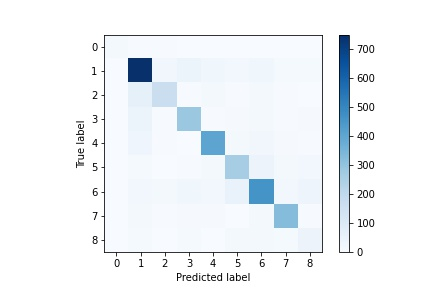
\includegraphics[scale=0.5]{cm_bert_clf_l1.jpg}
  \caption{\label{fig: F25} Covariance Matrix of BERT - Level 1}
\end{figure}

\begin{figure}[hb!]
  \centering
  \begin{subfigure}[b]{0.475\textwidth}
      \centering
      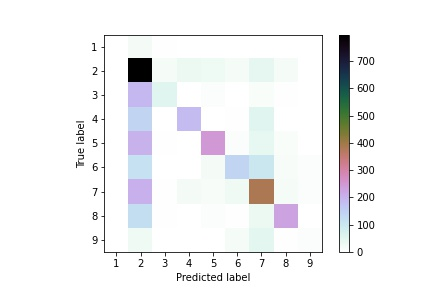
\includegraphics[width=\textwidth]{cm_word2vec_without_LR.jpg}
      {{\small Word2vec\_I LR}}    
  \end{subfigure}
  \hfill
  \begin{subfigure}[b]{0.475\textwidth}   
    \centering 
    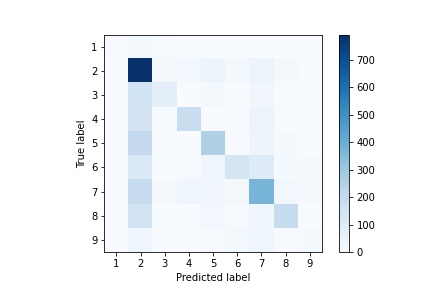
\includegraphics[width=\textwidth]{cm_word2vec_with_LR.jpg}
    {{\small Word2vec\_II LR}}    
  \end{subfigure}
  \vskip\baselineskip
  \begin{subfigure}[b]{0.475\textwidth}
    \centering
    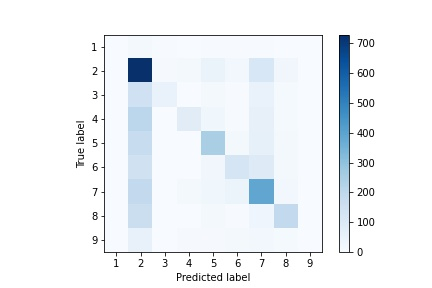
\includegraphics[width=\textwidth]{cm_doc2vec_without_LR.jpg}
    {{\small Doc2vec\_I LR}}    
\end{subfigure}
\hfill
\begin{subfigure}[b]{0.475\textwidth}   
  \centering 
  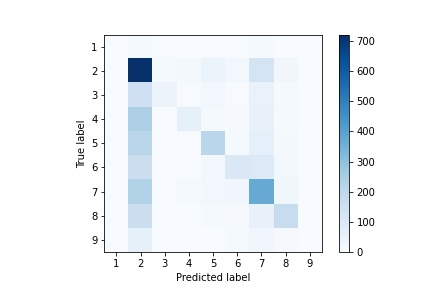
\includegraphics[width=\textwidth]{cm_doc2vec_with_LR.jpg}
  {{\small Doc2vec\_II LR}}    
\end{subfigure}
\caption{\label{fig: F23} Confusion Matrices Word2vec and Do2vec with and without Additional Knowldege Level 1 - LR}
\end{figure}

Besides this, the analysis does not explain the generally better performance of \ac{LR} and \ac{SVM} compared to \ac{RF} for the dense techniques and \ac{BERT}. One would expect \ac{RF} to perform better overall based on the imbalanced data. However, \ac{SVM} is said to handle large features better since they can learn independently of the dimensionality of the feature space. They are known to perform well for sparse vectors with a lot of relevant features, which is usually the case for text classification \citep{Joachims1998}. In addition for multi-class tasks, as mentioned in the literature review, often different versions of \ac{SVM} are used and showed good performance \citep{Aiolli2005, Angulo2003,Benabdeslem2006, guo2015, Mayoraz1999,Tang2019,tomar2015comparison}. \ac{LR} is preferred mainly for the sake of interpretability. A clear theoretical argument for the better performance of \ac{LR} in this application cannot be found. Ultimately, the results confirm previous findings in the literature. The performance of \ac{SVM} and especially of \ac{LR} might be due to the fact that \ac{LR} and \ac{SVM} simply work better with the data and the feature \citep{maglogiannis2007}. Considering the deep learning \ac{BERT} confusion matrix in figure \ref{fig: F25}, there seems to be no bias problem, which leaves the question of why does \ac{BERT} vectorizer with \ac{LR} work better? One explanation is the difference in the size of the data. The \ac{BERT} vectorizer was trained with much more data. The deep learning model probably performs better with the bigger dataset. However, the interpretability and transparency are lower compared to the \ac{BERT} vectorizer. As explained in the methods section, I controlled which pairs were given as input for the fine-tuning of the \ac{BERT} vectorizer and with what similarity, making it much more intuitive than the deep learning model that extracts features automatically. 

From the last comparison perspective, it is still unexplained why doc2vec\_II performed lower, and word2vec\_II performed slightly better. Figure \ref{fig: F23} reports the corresponding confusion matrices for \ac{LR}. The share of predictions and the correct predictions are reported in the appendix \ref{sec:B}. Considering word2vec, there are no considerable differences. Both models seem to be biased to the same extent using \ac{LR}. The same holds for \ac{RF}. Only when using \ac{SVM}, the bias for word2vec\_II seems to have slightly decreased. The correponding matrices are reported in the appendix. Thus, the slight variation between both models might be due to the additional knowledge. In contrast, doc2vec\_II has more predictions with label $2$ belonging to other labels. Therefore, the additional knowledge in the doc2vec model might be somewhat more biased, or adding the additional knowledge is harmful to the doc2vec vectorizer. 

\subsubsection*{Possible Explanations for Level 3 Results}
Looking at figure \ref{fig: F9} and the fact that level 3 reveals quite the same trends for the classifiers and methods as level 1, it is reasonable to assume that the classifiers of level 3 suffer from the same problem. However, the considerably higher number of classes makes it challenging to examine the bias visually, as was done for level 1 for the first two analyses. Instead, only the confusion matrices are studied.

According to the trends of level 3 and the explanations for level 1, it can be expected that the classifiers \ac{LR} and \ac{SVM} in combination with the sparse techniques as well as word2vec and doc2vec show a tendency towards imbalanced labels. This bias should be more apparent with doc2vec and word2vec. \ac{BERT}, in comparison, should be less biased or not biased at all. Figure \ref{fig: F21} shows the respective confusion matrices for \ac{LR}. For readability, the class labels are removed. The predicted labels for word2vec and doc2vec indeed show clearly two vertical lines, which indicates a bias. While the predictions for the count vectorizer for one label seem to be biased as well, the \ac{BERT} vectorizer again does not suffer from the imbalance of the training data. Further comparing the confusion matrices of level 1 over all classifiers to level 3 \ac{LR} matrices, except for \ac{BERT}, the diagonal line is not visible. This observation reflects the poor performance of the sparse techniques, word2vec and doc2vec and the excellent performance of \ac{BERT}. The confusion matrices of \ac{SVM} look similar to those of \ac{LR}, except of word2vec, where the bias can be partially identified for different labels. The respective matrix is given in the appendix \ref{sec:C}

\begin{figure}
  \centering
  \begin{subfigure}[b]{0.475\textwidth}
      \centering
      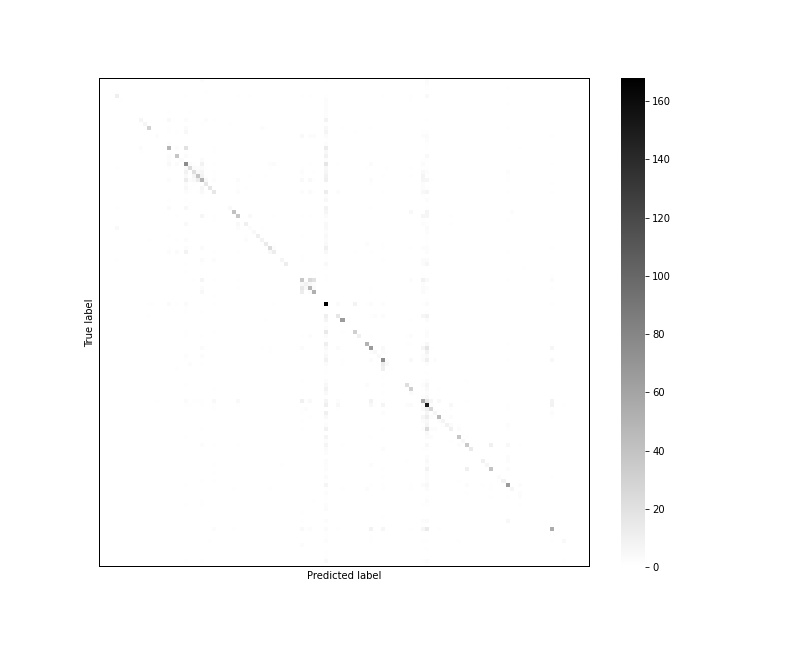
\includegraphics[width=\textwidth]{cm_count_LR_3.jpg}
      {{\small Count Vectorizer }}    
  \end{subfigure}
  \hfill
  \begin{subfigure}[b]{0.475\textwidth}  
      \centering 
      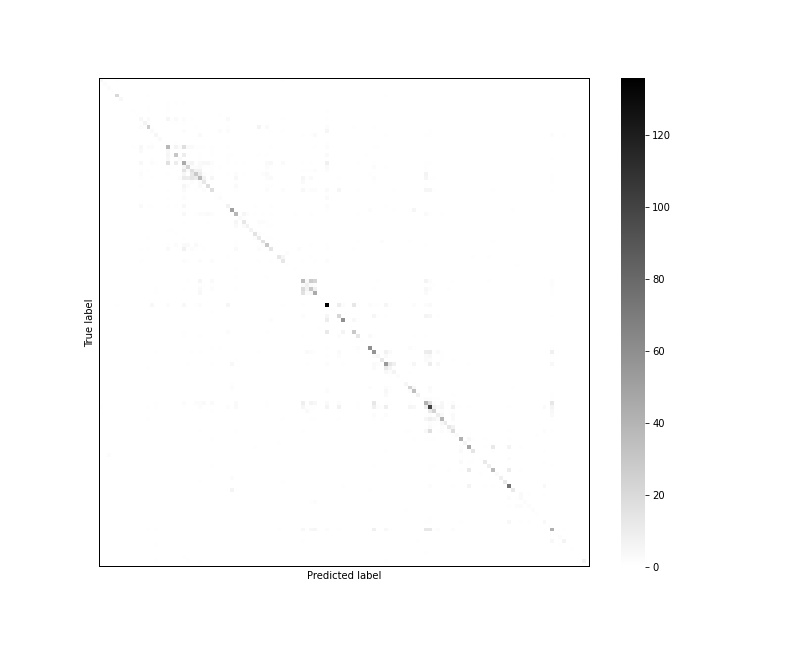
\includegraphics[width=\textwidth]{cm_bert_LR_3.jpg}
      {{\small BERT}}    
  \end{subfigure}
  \vskip\baselineskip
  \begin{subfigure}[b]{0.475\textwidth}   
    \centering 
    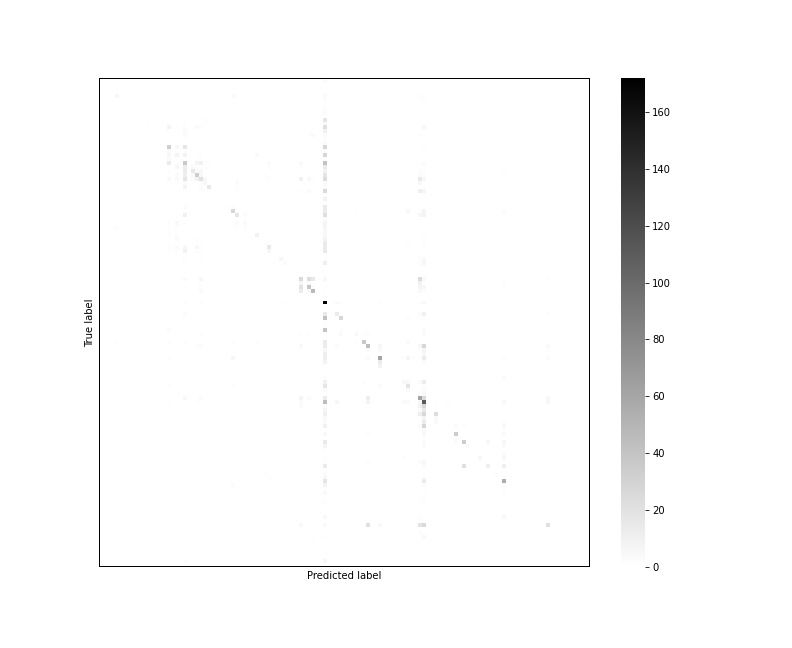
\includegraphics[width=\textwidth]{cm_word2vec_without_LR_3.jpg}
    {{\small Word2vec\_I}}    
  \end{subfigure}
  \hfill
  \begin{subfigure}[b]{0.475\textwidth}   
      \centering 
      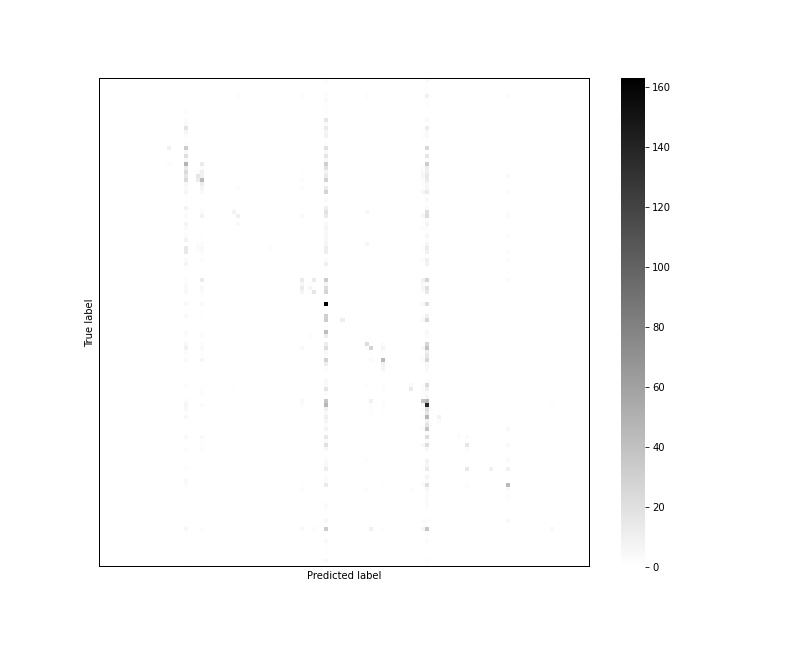
\includegraphics[width=\textwidth]{cm_doc2vec_without_LR_3.jpg}
      {{\small Doc2vec\_I}}    
  \end{subfigure}
  \caption{\label{fig: F21} Confusion Matrices Level 3 - LR}
\end{figure}


\begin{figure}
  \centering
  \begin{subfigure}[b]{0.475\textwidth}
      \centering
      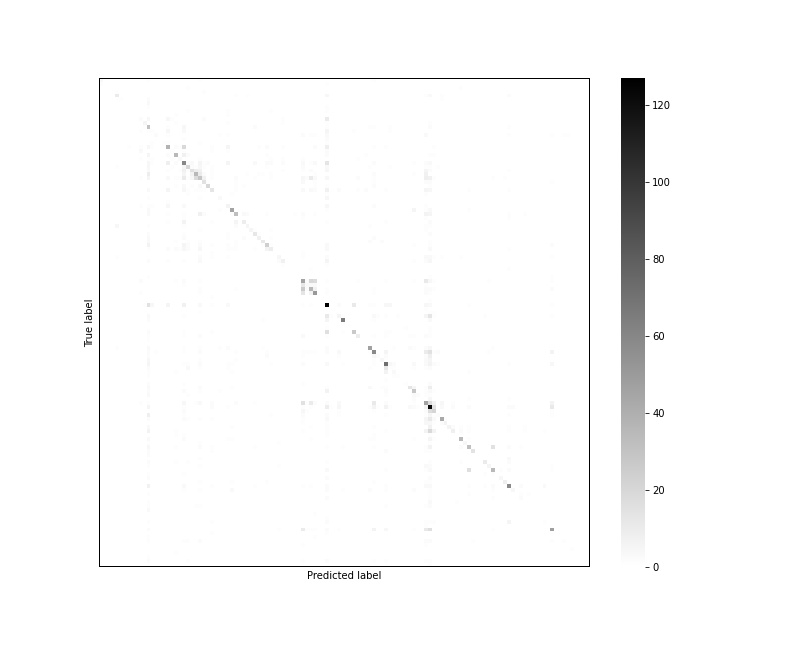
\includegraphics[width=\textwidth]{cm_count_RF_3.jpg}
      {{\small Count Vectorizer }}    
  \end{subfigure}
  \hfill
  \begin{subfigure}[b]{0.475\textwidth}  
      \centering 
      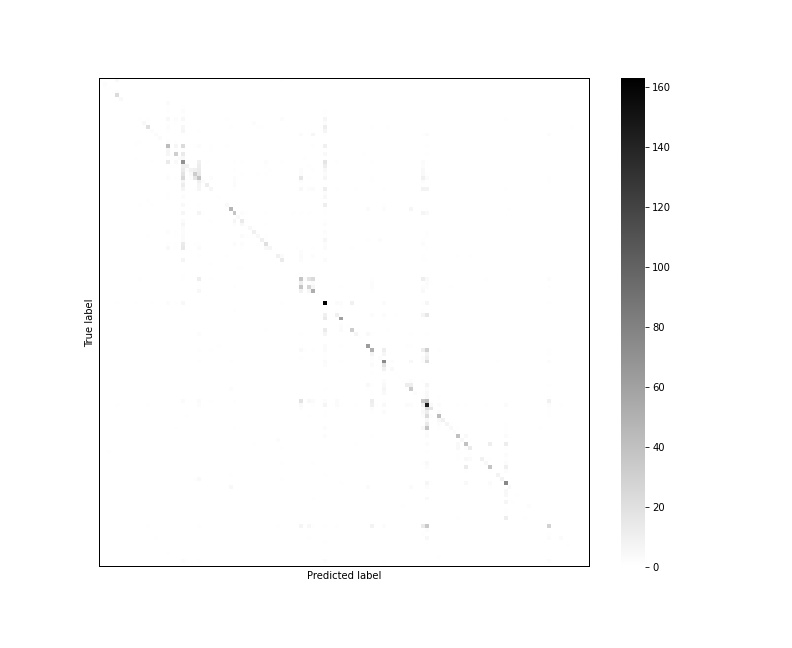
\includegraphics[width=\textwidth]{cm_bert_RF_3.jpg}
      {{\small BERT}}    
  \end{subfigure}
  \vskip\baselineskip
  \begin{subfigure}[b]{0.475\textwidth}   
    \centering 
    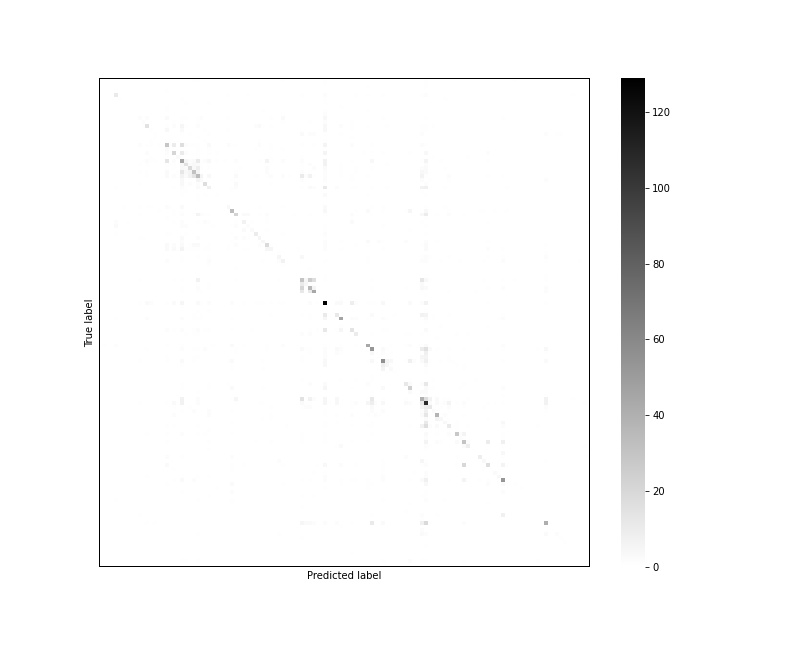
\includegraphics[width=\textwidth]{cm_word2vec_without_RF_3.jpg}
    {{\small Word2vec\_I}}    
  \end{subfigure}
  \hfill
  \begin{subfigure}[b]{0.475\textwidth}   
      \centering 
      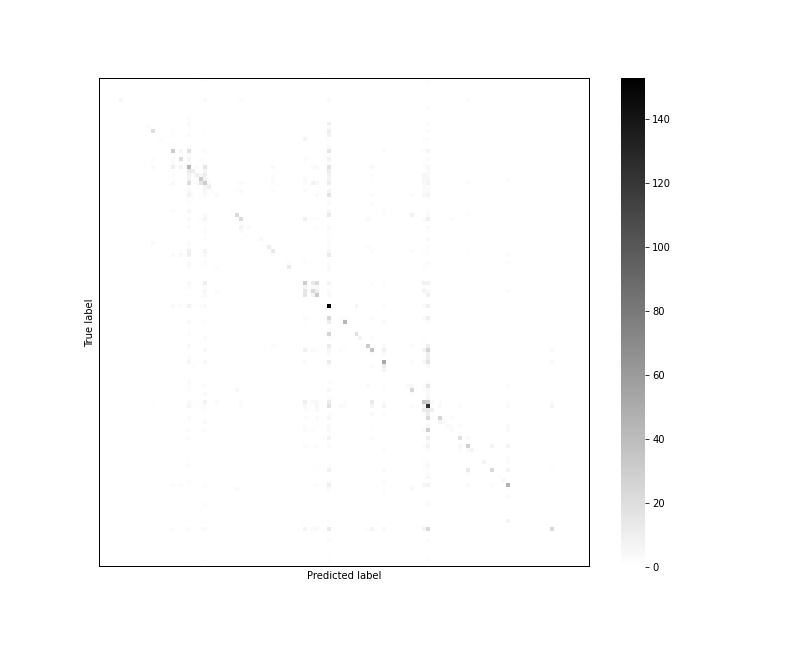
\includegraphics[width=\textwidth]{cm_doc2vec_without_RF_3.jpg}
      {{\small Doc2vec\_I}}    
  \end{subfigure}
  \caption{\label{fig: F22} Confusion Matrices Level 3 - RF}
\end{figure}

Similar to level 1, the performance for \ac{RF} is, due to the better handling of imbalance, better for word2vec and doc2vec, which is reflected in their confusion matrices in figure \ref{fig: F22}. While the performance of word2vec and doc2vec are closer to the sparse techniques for \ac{RF} than for the linear techniques, the confusion matrices do not clearly show differences. In addition, it is interesting that \ac{BERT} has a considerably better performance with \ac{RF}, while the confusion matrices do not have substantial differences in terms of the bias. Thus, the differences between the results for \ac{RF} remain unexplained by the analysis.

As for level 1, the generally lower performance for \ac{RF} for \ac{BERT} and sparse vectors cannot be explained by the analysis and is probably because \ac{RF} is not as suitable for the application as \ac{LR} and \ac{SVM}. More interesting is the low performance of the deep learning model. The confusion matrix of the \ac{BERT} deep learning model reported in the appendix, however, shows no differences to the \ac{BERT} vectorizer confusion matrix in figure \ref{fig: F22}. As mentioned above, for level 1, the deep learning model trained with much less data might have a greater impact on a classification problem with much more labels. The pairs for the vectorization are also specifically tailored for level 3. According to the literature, this might be a better strategy than using a deep learning model with automatic feature selection for a small dataset. 

The additional knowledge models behave similarly to level 1. The confusion matrices do not provide any remarkable differences. Adding knowledge seems to improve the performance of word2vec somewhat, while it seems to be detrimental to doc2vec.


\section{Conclusion and Limitations}
The starting point of this work was to examine the classification of job titles of German job postings with the taxonomy \ac{KldB} 2010. Based on the literature on text classification and the challenges of short text classification, the analysis was conducted along three pillars: application of different vectorization techniques, training of different classification algorithms, and treatment of short job titles by adding additional knowledge. 

The results revealed some interesting trends. The \ac{BERT} vectorizer in combination with \ac{LR} has shown the best performance. Due to imbalanced data, the other classification algorithms might have developed a label bias in different settings, both for level 1 and level 3. \ac{RF} can reduce this bias for doc2vec and word2vec, but not to the extent that it overpowers the sparse vectors or \ac{BERT} results, especially in combination with the linear classification algorithms. The deep learning model of \ac{BERT} performs, in general and especially for level 3, worse than the \ac{BERT} vectorizer. Adding additional knowledge does not lead to clear improvement. The performance of word2vec seems to improve slightly, whereas that of doc2vec deteriorates slightly. 

In conclusion, this paper suggests that the \ac{BERT} vectorizer is, due to the stable and excellent performance in classifying imbalanced data and compared to the other methods, a promising method for classifying job titles into the \textit{kldb} classes, especially in combination with \ac{LR}. The possibility of controlling which pairs are used as input for the fine-tuning gives the \ac{BERT} vectorizer the advantage of being interpretable and transparent. Furthermore, there is much space for improvements with this vectorizer method. Future research could combine pairs in other ways, for instance by including the label names of the \textit{kldb} or by combining search words for different levels with different probabilities. This would result in vast datasets with millions of pairs for the fine-tuning process. However, corresponding computing resources must then also be available for the training process. 

The results of this study are subject to several limitations that need to be addressed in future research to develop a high-performance classification algorithm. The first limitation concerns the dataset. As detailed in the discussion of the results, the data imbalance has been problematic for most methods. This was reflected in the performance, especially for level 3, where many classes have few to no examples. Due to this fact, it was also not possible to train all taxonomy classes - 8 out of the 144 classes on level 3 were not trained. For level 1, class 0 could not be trained. In addition, this problem led to ill-defined metrics, which in part only allowed a cautious interpretation of the performance. Further, only a sample of the dataset could be used in this work due to limited computational resources. A larger dataset is likely to improve the results, especially those of the deep learning model. Additionally, future research should investigate how to cope with the imbalanced data in order to compare the vectorization methods without the bias problem. Another strategy that should be pursued, is to enrich the data manually with examples for minority classes. Such efforts are also vital to ensure that all classes are trained.

The second limitation addresses the question of generalization. A frequent problem is overfitting the classifier to the trainings data. The data was divided into training and test data to ensure that the performance was measured on unseen data. However, since not all classes are trained, the classifiers cannot classify titles belonging to those missing classes, restricting the generalizability of the algorithms. Furthermore, the classifiers are not multilingual and therefore cannot be generalized to job postings in other languages. 

Lastly, there is certainly room for improving the usage of additional knowledge. As \ac{BERT} is a promising technique, one could combine and compare different \ac{BERT} algorithms with additional knowledge. For example, \citet{ostendorff2019} use an approach of enriching \ac{BERT} with knowledge graph embeddings. This is a relevant topic for future work. 

\begin{figure}[hb!]
  \center
  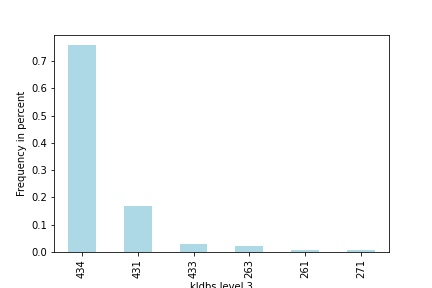
\includegraphics[scale=0.5]{kldbs_frequency_softwareentwickler.jpg}
  \caption{\label{fig: F27} Share of \textit{Kldb} for the Occupation `softwareentwickler"}
\end{figure}

\begin{figure}[hb!]
  \center
  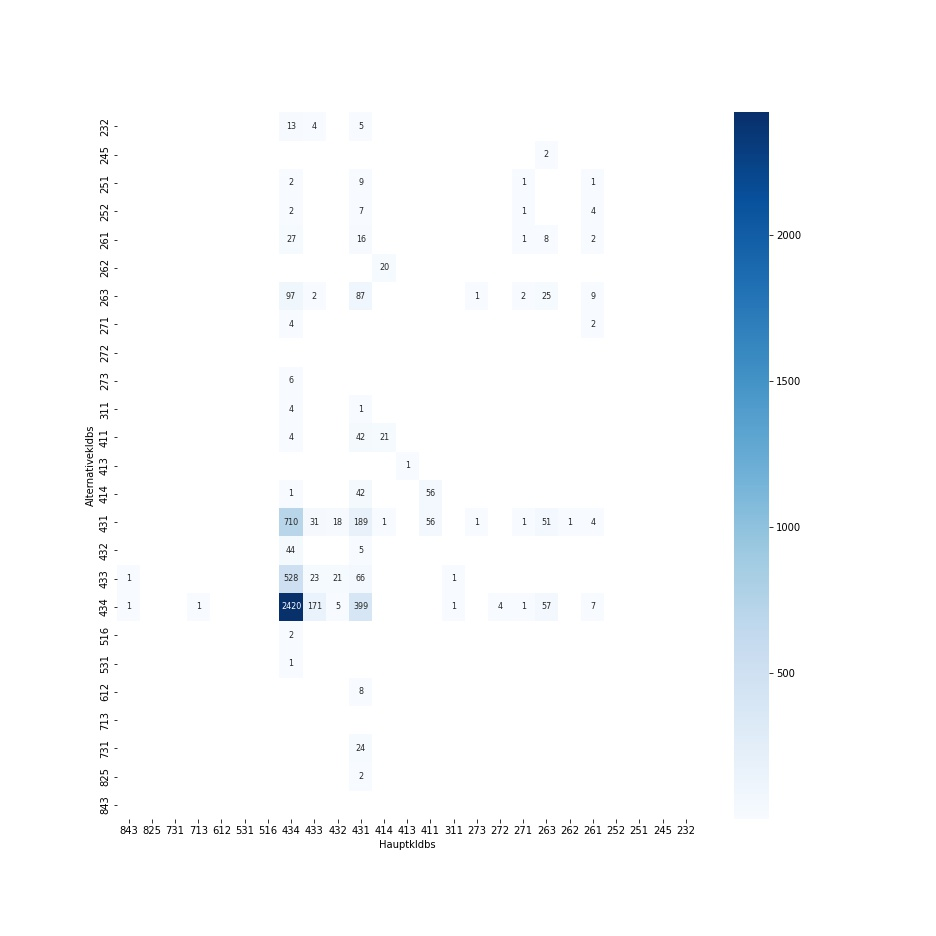
\includegraphics[scale=0.4]{co_occurence_softwareentwickler.jpg}
  \caption{\label{fig: F28} Co-occurence Matrix for the Occupation `softwareentwickler"}
\end{figure}

% \begin{figure}
%   \begin{subfigure}{.5\textwidth}
%     \centering
%     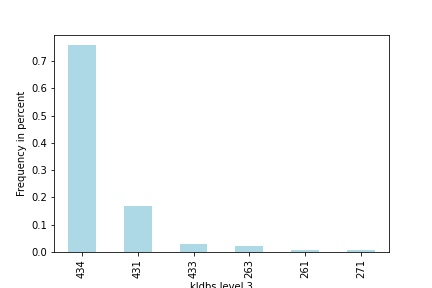
\includegraphics[width=.8\linewidth]{kldbs_frequency_softwareentwickler.jpg}
%     \caption{\label{fig: F27} Share of \textit{kldb} for the occupation `softwareentwickler"}
%   \end{subfigure}%
%   \begin{subfigure}{.5\textwidth}
%     \centering
%     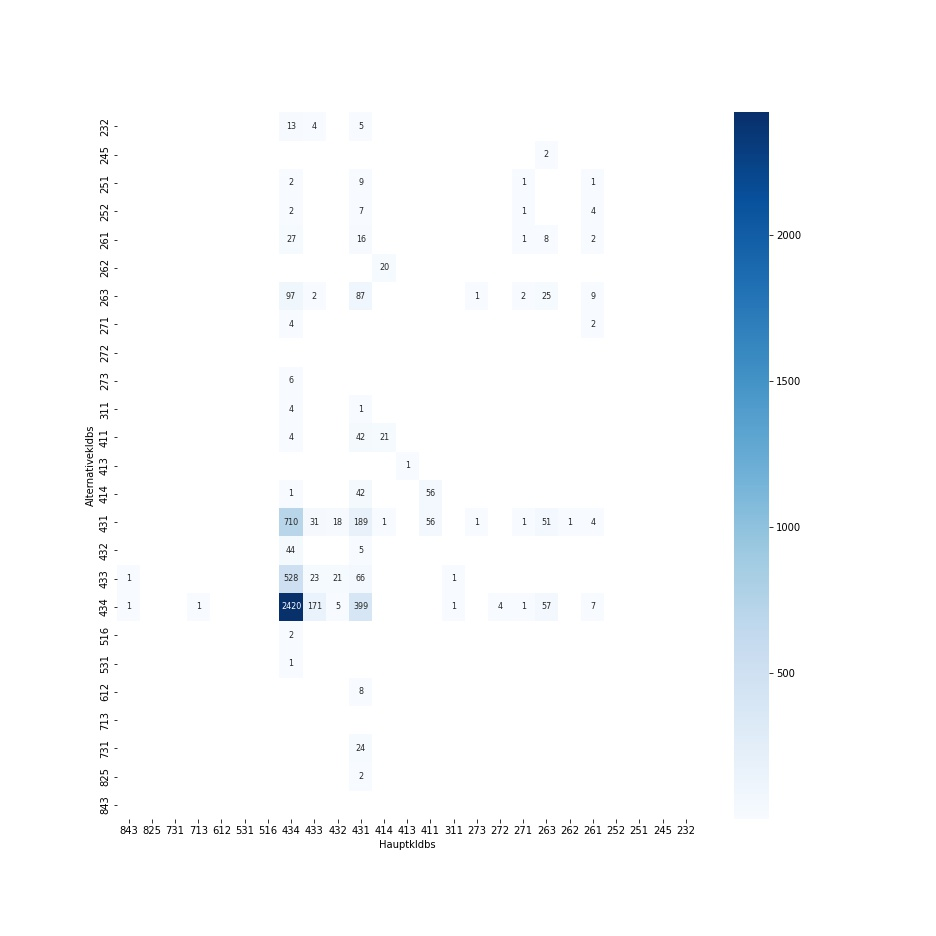
\includegraphics[width=.9\linewidth]{co_occurence_softwareentwickler.jpg}
%     \caption{\label{fig: F28} Co-occurence matrix for the occupation `softwareentwickler"}
%   \end{subfigure}
%   \end{figure}

In addition to the above limitations, in general, the complexity of structuring and normalizing job titles limits the ability to improve the performance of the job title classification algorithms. Considering the occupation software developer, figure \ref{fig: F27} shows the \textit{kldb} that are assigned to the title with the terms ``softwareentwickler" or ``softwareentwicklerin" in the training dataset. Most of the titles belong to ``434", but approx. $30\%$ are assigned to other \textit{kldbs}. Comparing the titles in these different \textit{kldbs}, most of them do not contain keywords other than ``Softwareentwickler" or ``Softwareentwicklerin" that would allow distinguishing the \textit{kldbs}. There are even titles with exactly the same wording in the different \textit{kldbs}. Thus, the data is ambiguous for some occupations and making it impossible for a classifier to differentiate between the \textit{kldbs}. This reveals the complexity of the problem and the limitations of improving in the performance. 
In addition to the above limitations, in general, the complexity of structuring and normalizing job titles limits the ability to improve the performance of the job title classification algorithms. Considering the occupation software developer, figure \ref{fig: F27} shows the \textit{kldb} that are assigned to the title with the terms ``softwareentwickler" or ``softwareentwicklerin" in the training dataset. Most of the titles belong to ``434", but approx. $30\%$ are assigned to other \textit{kldb}. Comparing the titles in these different \textit{kldbs}, most of them do not contain keywords other than ``Softwareentwickler" or ``Softwareentwicklerin" that would allow distinguishing the \textit{kldbs}. There are even titles with exactly the same wording in the different \textit{kldbs}. Thus, the data is ambiguous for some occupations and \textit{kldb} making it impossible for a classifier to differentiate between the \textit{kldb}. This reveals the complexity of the problem and the limitations of improving in the performance. 

The problem just highlighted raises the question of whether the limitation is merely a problem of the quality of the dataset. This can be clarified by analyzing the alternative \textit{kldbs} that employers can provide in case of uncertainty. The heatmap in \ref{fig: F28} shows on the horizontal line the \textit{kldbs} which were used for the training and on the vertical line the alternative \textit{kldbs}. Considering again the main \textit{kldb} $431$, the vertical line that emanates from this \textit{kldb} indicates that it is not clear at all what \textit{kldb} a title might belong in the real world.\footnote{Note that this analysis relies on the complete dataset, not on the short one. This is due to illustrative purposes to highlight the problem better. However, since a sample with the same distribution was drawn, the logic is the same.} This poses the question of whether it is adequate to develop a classifier with only one class as an output. At the same time, one should elaborate on whether a multilabel classification algorithm is practical for downstream tasks in this domain. In addition, there are concerns about appropriate evaluation measurements. This may constitute the object of future studies.

In spite of this limitations, this paper is the first step towards establishing a job title classification system for German job postings with the \ac{KldB} by providing initial results and first analysis. The results on \ac{BERT} and the problem of biased classifiers are leading the way for future research.

\newpage

\begin{ConflictofInterest}
The paper was written as part of a project by cause\&effect DFSG UG, which collaborates with the Bertelsmann Foundation. The data for this work was provided by cause\&effect DFSG UG. The work was not financially supported neither by cause\&effect DFSG UG nor by the Bertelsmann Foundation. The interests of both parties did not influence the results of this study. I, therefore, declare that there have been no conflicts of interest.
\end{ConflictofInterest}

\newpage

\pagenumbering{roman}
\bibliographystyle{apalike}
\bibliography{exportV1}

\clearpage
\pagenumbering{arabic}
\renewcommand*{\thepage}
{A\arabic{page}}
\appendix
\section{Data}
\label{sec:A}
\subsection*{Data Snippet Raw Data}
\begin{lstlisting}[language=json]
  {
    "hashId": "-IgNS05-jeri5aZhe0_VK35Y0-6xQAoADg3b0MyraTI=",
    "hauptberuf": "Telefonist/in",
    "freieBezeichnung": "Telefonist / Telefonistin m/w/d",
    "referenznummer": "14469-20210617140207-S",
    "mehrereArbeitsorteVorhanden": false,
    "arbeitgeber": "aventa Personalmanagement GmbH",
    "arbeitgeberHashId": "MYRG2meMKxCjrQ9Cpl8JwgEDPbM133Z9iRCkolaOONo=",
    "aktuelleVeroeffentlichungsdatum": "2021-06-29",
    "eintrittsdatum": "2021-06-29",
    "logoHashId": "wMN78p7yNK_C0aJDJ77l63RVH3DCEzwJGxZk1ZzsUrY=",
    "angebotsart": "ARBEIT",
    "hauptDkz": "7389",
    "alternativDkzs": [
      "35082"
    ],
    "angebotsartGruppe": "ARBEIT",
    "anzeigeAnonym": false,
    "arbeitsort": {
      "plz": "10407",
      "ort": "Berlin",
      "region": "Berlin",
      "land": "Deutschland",
      "koordinaten": {
        "lat": 52.5335379,
        "lon": 13.4462856
      }
    },
    "_links": {
      "details": {
        "href": "http://jobboerse.arbeitsagentur.de/vamJB/stellenangebotAnzeigen.html?bencs=xZ8NQKDByg2g6avJgLLIrGwqlXZQi1GKNAI%2BzAoCWJ5RD6egZDnwqMFj%2B4AnUX6XN5nyEJ7NKSdBBr1EvlmnVw%3D%3D"
      },
      "arbeitgeberlogo": {
        "href": "https://api-con.arbeitsagentur.de/prod/jobboerse/jobsuche-service/ed/v1/arbeitgeberlogo/wMN78p7yNK_C0aJDJ77l63RVH3DCEzwJGxZk1ZzsUrY="
      },
      "jobdetails": {
        "href": "https://api-con.arbeitsagentur.de/prod/jobboerse/jobsuche-service/pc/v1/jobdetails/-IgNS05-jeri5aZhe0_VK35Y0-6xQAoADg3b0MyraTI="
      }
    }
  },
\end{lstlisting}


\subsection*{Snippet of Trainingsdata (without Preprocessing) - Level 1}
\begin{lstlisting}[language=json, firstnumber=1]
{'id': '2', 'title': 'Maschinenbediener (m/w/d)'}
{'id': '7', 'title': 'Controlling'}
{'id': '5', 'title': 'Lagermitarbeiter (m/w/d)'}
{'id': '2', 'title': 'Reifenmonteur (m/w/d) Facharbeiter'}
{'id': '5', 'title': 'Kommissionierer (m /w /d)'}
{'id': '7', 'title': 'Sachbearbeiter (m/w/d) im Einkauf Weimar'}
{'id': '5', 'title': 'Schubmaststapler Fahrer (m/w/d)'}
{'id': '3', 'title': 'Bauhelfer Elektroinstallation (m/w/d)'}
{'id': '7', 'title': 'Telefonist / Telefonistin m/w/d'}
{'id': '9', 'title': 'Telefonische Kundenbetreuung (m/w/d)'}
\end{lstlisting}


\subsection*{Snippet of Trainingsdata (Preprocessed) - Level 1}
\begin{lstlisting}[language=json, firstnumber=1]
[{'id': '2', 'title': 'maschinenbediener'},
 {'id': '7', 'title': 'controlling'},
 {'id': '5', 'title': 'lagermitarbeiter'},
 {'id': '2', 'title': 'reifenmonteur facharbeiter'},
 {'id': '5', 'title': 'kommissionierer'},
 {'id': '7', 'title': 'sachbearbeiter einkauf weimar'},
 {'id': '5', 'title': 'schubmaststapler fahrer'},
 {'id': '3', 'title': 'bauhelfer elektroinstallation'},
 {'id': '7', 'title': 'telefonist telefonistin'},
 {'id': '9', 'title': 'telefonische kundenbetreuung'}]
\end{lstlisting}

\subsection*{Class Distribution of Level 1 und Level 3 (complete Dataset)}
\begin{figure}[hb!]
  \begin{subfigure}{.5\textwidth}
    \centering
    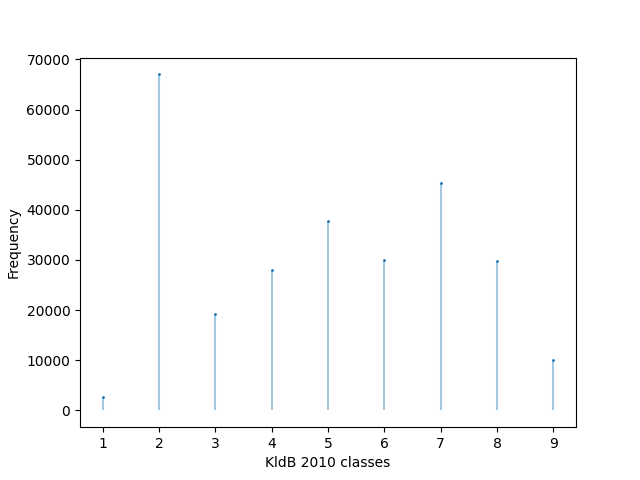
\includegraphics[width=.9\linewidth]{training_data_long_L1.png}
    \caption{\label{fig: F11} Class Distribution Level 1}
  \end{subfigure}%
  \begin{subfigure}{.5\textwidth}
    \centering
    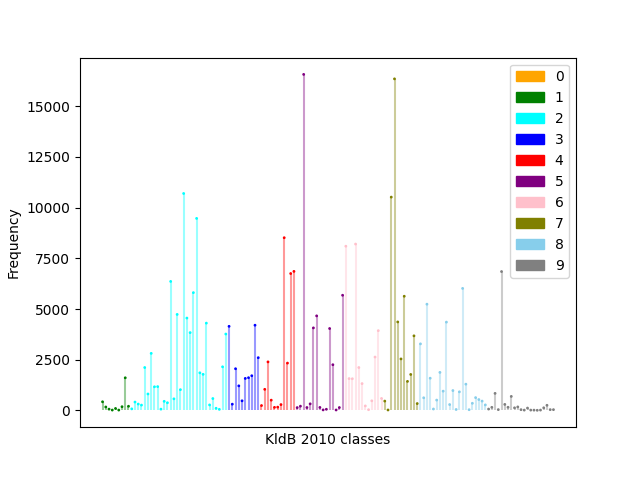
\includegraphics[width=.9\linewidth]{training_data_long_L3.png}
    \caption{\label{fig: F12} Class Distribution Level 3}
  \end{subfigure}
  \caption{Class Distribution of Training Data}
  \end{figure}

  \newpage

\section{Prediction Results- Level 1}
\label{sec:B}
\subsection*{Predictions - SVM}
\begin{figure}[hb!]
  \centering
  \begin{subfigure}[b]{0.475\textwidth}
      \centering
      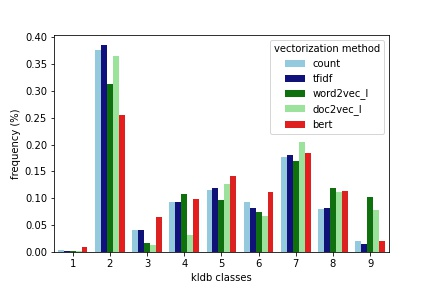
\includegraphics[width=\textwidth]{predictions_SVM_L1.jpg}
      {
        {\bigskip
          \small Share of predictions labels for level 1 - SVM}
      }    
  \end{subfigure}
  \hfill
  \begin{subfigure}[b]{0.475\textwidth}  
      \centering 
      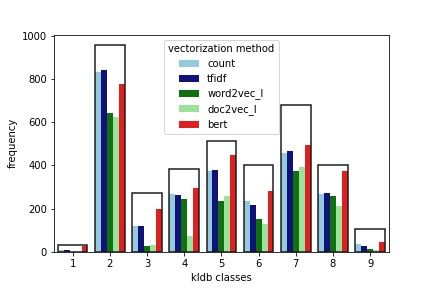
\includegraphics[width=\textwidth]{predictions_correct_relative_SVM_L1.jpg}
      {{\small Frequency of correct predictions for each labels and frequency of true labels - SVM}}    
  \end{subfigure}
\caption{Predictions Level 1- SVM}
\end{figure}

\newpage

\subsection*{Confusion Matrices for all Vectorization Techniques - SVM}
\begin{figure}[hb!]
  \centering
  \begin{subfigure}[b]{0.475\textwidth}  
    \centering 
    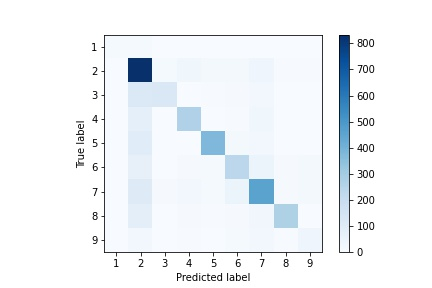
\includegraphics[width=\textwidth]{cm_count_SVM_L1.jpg}
    {{\small Count Vectorizer SVM}}    
  \end{subfigure}
  \hfill
  \begin{subfigure}[b]{0.475\textwidth}   
      \centering 
      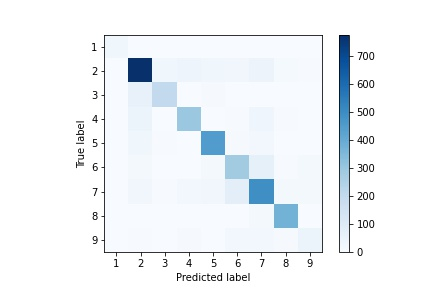
\includegraphics[width=\textwidth]{cm_bert_SVM_L1.jpg}
      {{\small BERT}}    
  \end{subfigure}  
  \vskip\baselineskip
  \begin{subfigure}[b]{0.475\textwidth}  
    \centering 
    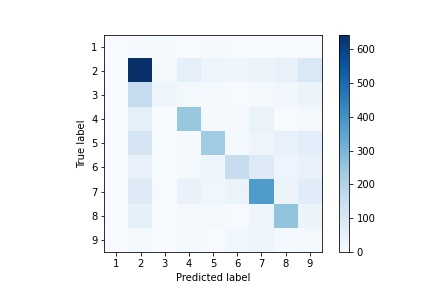
\includegraphics[width=\textwidth]{cm_word2vec_without_SVM_L1.jpg}
    {{\small Word2vec\_I SVM}}    
  \end{subfigure}
  \hfill
  \begin{subfigure}[b]{0.475\textwidth}   
      \centering 
      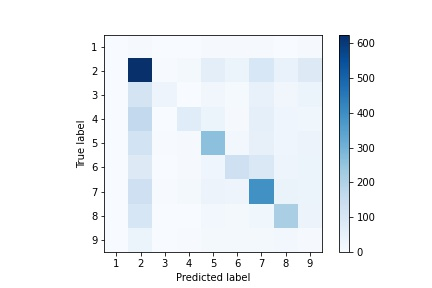
\includegraphics[width=\textwidth]{cm_doc2vec_without_SVM_L1.jpg}
      {{\small Doc2vec\_I SVM}}    
  \end{subfigure}
  \vskip\baselineskip
  \begin{subfigure}[b]{0.475\textwidth}  
    \centering 
    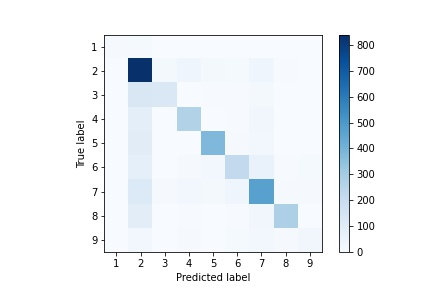
\includegraphics[width=\textwidth]{cm_tfidf_SVM_L1.jpg}
    {{\small Word2vec\_I SVM}}    
  \end{subfigure}
  \caption{Confusion Matrices for all Vectorization Techniques - SVM}
\end{figure}

\newpage
\FloatBarrier
\subsection*{Confusion matrices TF-IDF - LR and RF}
\begin{figure}[hb!]
  \centering
  \begin{subfigure}[b]{0.475\textwidth}
      \centering
      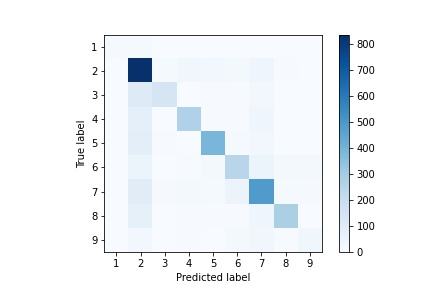
\includegraphics[width=\textwidth]{cm_tfidf_LR_L1.jpg}
      {{\small TF-IDF LR}}    
  \end{subfigure}
  \hfill
  \begin{subfigure}[b]{0.475\textwidth}  
      \centering 
      \includegraphics[width=\textwidth]{cm_tfidf_RF_L1.jpg}
      {{\small TF-IDF RF}}    
  \end{subfigure}
\caption{TF-IDF RF}
\end{figure}

\subsection*{Predictions of word2vec and doc2vec with additional knowledge}
\begin{figure}[hb!]
  \centering
  \begin{subfigure}[b]{0.475\textwidth}  
    \centering 
    \includegraphics[width=\textwidth]{predictions_correct_relative_word_doc_LR.jpg}
    {{\small Predictions additional knowledge - LR}}    
  \end{subfigure}
  \hfill
  \begin{subfigure}[b]{0.475\textwidth}   
      \centering 
      \includegraphics[width=\textwidth]{predictions_correct_relative_word_doc_RF.jpg}
      {{\small Predictions additional knowledge - RF}}    
  \end{subfigure}  
  \vskip\baselineskip
  \begin{subfigure}[b]{0.475\textwidth}  
    \centering 
    \includegraphics[width=\textwidth]{predictions_correct_relative_word_doc_SVM.jpg}
    {{\small Predictions additional knowledge - SVM}}    
  \end{subfigure}
  \caption{Predictions additional knowledge for all classifiers}
\end{figure}

\newpage

\subsection*{Confusion Matrices Word2vec and Doc2vec - Additional Knowledge - SVM}
\begin{figure}[hb!]
  \centering
  \begin{subfigure}[b]{0.475\textwidth}  
    \centering 
    \includegraphics[width=\textwidth]{cm_word2vec_without_SVM_L1.jpg}
    {{\small word2vec\_I SVM}}    
  \end{subfigure}
  \hfill
  \begin{subfigure}[b]{0.475\textwidth}   
      \centering 
      \includegraphics[width=\textwidth]{cm_word2vec_with_SVM_L1.jpg}
      {{\small word2vec\_II SVM}}    
  \end{subfigure}  
  \vskip\baselineskip
  \begin{subfigure}[b]{0.475\textwidth}  
    \centering 
    \includegraphics[width=\textwidth]{cm_doc2vec_without_SVM_L1.jpg}
    {{\small doc2vec\_I SVM}}    
  \end{subfigure}
  \hfill
  \begin{subfigure}[b]{0.475\textwidth}   
      \centering 
      \includegraphics[width=\textwidth]{cm_doc2vec_with_SVM_L1.jpg}
      {{\small doc2vec\_II SVM}}    
  \end{subfigure}
  \caption{Confusion Matrices Word2vec and Doc2vec With and Without Additional Knowldege Level 1 - SVM}
\end{figure}

\newpage

\FloatBarrier
\subsection*{Confusion Matrices Word2vec and Doc2vec - Additional Knowledge - RF}
\begin{figure}[hb!]
  \centering
  \begin{subfigure}[b]{0.475\textwidth}  
    \centering 
    \includegraphics[width=\textwidth]{cm_word2vec_without_RF.jpg}
    {{\small word2vec\_I RF}}    
  \end{subfigure}
  \hfill
  \begin{subfigure}[b]{0.475\textwidth}   
      \centering 
      \includegraphics[width=\textwidth]{cm_word2vec_with_RF.jpg}
      {{\small word2vec\_II RF}}    
  \end{subfigure}  
  \vskip\baselineskip
  \begin{subfigure}[b]{0.475\textwidth}  
    \centering 
    \includegraphics[width=\textwidth]{cm_doc2vec_without_RF.jpg}
    {{\small doc2vec\_I RF}}    
  \end{subfigure}
  \hfill
  \begin{subfigure}[b]{0.475\textwidth}   
      \centering 
      \includegraphics[width=\textwidth]{cm_doc2vec_with_RF.jpg}
      {{\small doc2vec\_II RF}}    
  \end{subfigure}
  \caption{Confusion Matrices Word2vec and Doc2vec With and Without Additional Knowldege Level 1 - RF}
\end{figure}

\newpage
\section{Prediction Results- Level 3}
\label{sec:C}
\subsection*{Confusion Matrix - BERT Deep Learning Model}
\begin{figure}[hb!]
  \center
  \includegraphics[scale=0.5]{cm_bert_clf_3.jpg}
  \caption{Confusion Matrix - BERT Deep Learning Model}
\end{figure}

\newpage
\subsection*{Confusion matrices TF-IDF - LR and RF}
\begin{figure}[hb!]
  \centering
  \begin{subfigure}[b]{0.475\textwidth}  
    \centering 
    \includegraphics[width=\textwidth]{cm_tfidf_LR.jpg}
    {{\small TF-IDF - LR}}    
  \end{subfigure}
  \hfill
  \begin{subfigure}[b]{0.475\textwidth}   
      \centering 
      \includegraphics[width=\textwidth]{cm_tfidf_RF.jpg}
      {{\small TF-IDF - RF}}    
  \end{subfigure}  
  \caption{Confusion Matrices TF-IDF - LR and RF}
\end{figure}

\newpage
\subsection*{Confusion Matrices for all Vectorization Techniques - SVM}
\begin{figure}[hb!]
  \centering
  \begin{subfigure}[b]{0.475\textwidth}  
    \centering 
    \includegraphics[width=\textwidth]{cm_count_SVM.jpg}
    {{\small Count Vectorizer SVM}}    
  \end{subfigure}
  \hfill
  \begin{subfigure}[b]{0.475\textwidth}   
      \centering 
      \includegraphics[width=\textwidth]{cm_bert_SVM.jpg}
      {{\small BERT}}    
  \end{subfigure}  
  \vskip\baselineskip
  \begin{subfigure}[b]{0.475\textwidth}  
    \centering 
    \includegraphics[width=\textwidth]{cm_word2vec_without_SVM.jpg}
    {{\small Word2vec\_I SVM}}    
  \end{subfigure}
  \hfill
  \begin{subfigure}[b]{0.475\textwidth}   
      \centering 
      \includegraphics[width=\textwidth]{cm_doc2vec_without_SVM.jpg}
      {{\small Doc2vec\_I SVM}}    
  \end{subfigure}
  \vskip\baselineskip
  \begin{subfigure}[b]{0.475\textwidth}  
    \centering 
    \includegraphics[width=\textwidth]{cm_tfidf_SVM.jpg}
    {{\small Word2vec\_I SVM}}    
  \end{subfigure}
  \caption{Confusion Matrices for all Vectorization Techniques - SVM}
\end{figure}

\end{document}
